\documentclass[binding=0.7cm, oneside]{sapthesis}

\usepackage{microtype}
\usepackage{hyperref}
\usepackage {subcaption}
\usepackage{enumitem}
\hypersetup{pdftitle={My thesis},pdfauthor={Francesco Danese}}

\title{A Robust Person Identification Method Through Wi-Fi Signals}
\author{Francesco Danese}
\IDnumber{1926188}
\course{Applied Computer Science and Artificial Intelligence}
\courseorganizer{Faculty of Information Engineering, Informatics, and Statistics}
\AcademicYear{2022/2023}
\advisor{Prof. Luigi Cinque}
\coadvisor{Prof. Danilo Avola}
\coadvisor{Prof. Daniele Pannone}
\copyyear{2023}
\authoremail{francescodanese01@gmail.com}
\begin{document}
\frontmatter
\maketitle

\begin{abstract}
    This thesis deals with myself.
\end{abstract}

\tableofcontents
\mainmatter
\chapter{Introduction}
In the last years, Wi-Fi technology is turning into a ubiquitous and fundamental tool, not only for providing
constant and easy-access internet connection but also for enabling the development of the Internet of Things and
radio-based sensing applications. Cutting-edge Wi-Fi sensing systems use wireless signals to detect events or changes,
such as motion and gesture recognition \cite{gesture_recognition}, in the permeated environment leveraging the disturbances
and variations in the received radio signal. In this work, Wi-Fi sensing technology is employed for person Identification, a task
usually achieved by vision-based systems through the use of RGB cameras. In common scenarios, person Identification is a classification
task where the input features, such as an image or a video of a particular individual, is examined in order to recognize him among a specific
set of people. To reach this goal, in modern approaches the raw input image is analyzed in order to model a person appearance and physical
constitution, by extracting some key features that will be use for inference, as shown in Fig. \ref{fig:visionID}. State-of-the-art methods include leveraging deep learning models
trained to identify a human, like: Convolutional Neural Network for detecting the face of the person \cite{cnn_face_id} and recognize him;
Recurrent Neural Networks \cite{Recurrent_nn_reid} and their variants, such as LSTMs, for working with sequences of data like video sequences
and exploiting the unique person behavior like the walking gait \cite{Gait_cnn}; Attention mechanisms, as seen in models like Transformers \cite{Transformers_reid},
for their ability to focus on relevant parts of an image or sequence therefore locating the discriminative features.
Although vision-based methods have achieved remarkable results, several issues arise during real-world scenarios, including:
subject occlusion and pose; different viewing angles and image scale; ambient changes in illumination; modifications in personal look
(clothes, haircut, glasses) and privacy concerns due to the sensitive nature of personal imaging data. To address these challenges,
a non-conventional approach can be adopted, that walks away from images and vision avoiding the aforementioned issues, through the use of
completely different types of data: Wi-Fi signals.
\begin{figure}[h!]
    \centering
    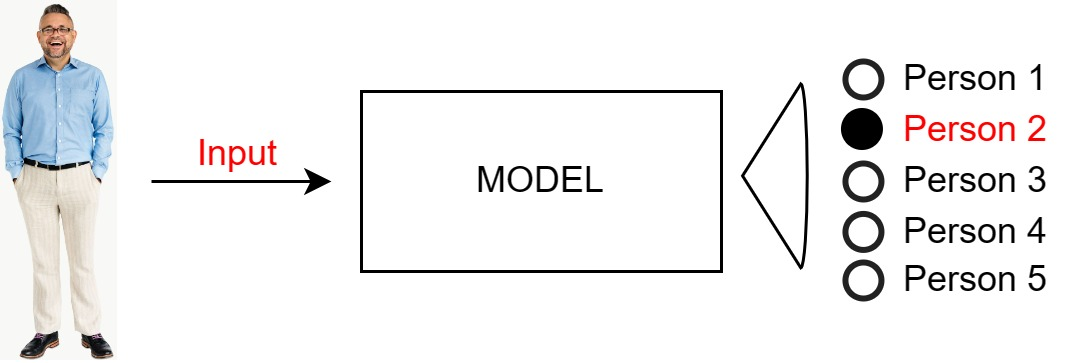
\includegraphics[scale=0.3]{images/Person_id.jpg}
    \caption{Image-based person ID within a group of 5 people.}
    \label{fig:visionID}
\end{figure}

Wi-Fi technology has revolutionized the way we connect and communicate in the digital age. It enables wireless communication between devices by
utilizing radio signals transmitted by access points (APs). The signals can be influenced by various factors, such as objects and people,
leading to signal variations along their path. These variations, essential for understanding the wireless environment,
are captured through measurements like the Received Signal Strength Indicator (RSSI) and Channel State Information (CSI),
which play a pivotal role in implementing wireless sensing applications. The RSSI serves as a measure of the reduction in the strength of radio signals
as they travel through space, capturing the way signals diminish over distance. Even though this metric has found widespread utilization within numerous
indoor localization systems \cite{RSSI_indoorloc,RSSI_indoorloc_new}, which goal is to find where a certain target is in an enclosed location with meter-precision,
it experiences unsustainable performance drops in complex situations, due to several limitations. The problems associated with RSSI stem from its simplicity and
lack of granularity, which restrict its ability to capture detailed signal characteristics and changes accurately. In fact, for a given wireless data packet, RSSI
provides a single value computed at MAC layer, that represents the overall signal strength, without differentiating between the effects of multipath interference,
signal reflections, or other external factors. Moreover, the relationship between RSSI values and the real signal strength is often non-linear, so that small changes
in RSSI may not correspond to proportional changes in signal strength, making it challenging to interpret signal variations accurately. For these relevant reasons, RSSI fails
to provide detailed insights into how the signal interacts with the surrounding environment \cite{RSSI_reliability_indoorloc}. On the other hand, the CSI is derived
from the PHY layer's orthogonal frequency-division multiplexing (OFDM) transmission technology and includes detailed signal information defined at the subcarrier level,
making it more stable and capable of carrying a higher level of signal information. CSI measurements offer access to a broader range of signal properties, including
amplitude and phase for each subcarrier, providing higher granularity than RSSI \cite{CSI_RSSI}. Furthermore, CSI can be computed using commodity Wi-Fi devices,
making it a popular choice in Wireless sensing applications. To ensure the quality of received CSI measurements, signal pre-processing techniques are often employed,
such as removing amplitude outliers and phase offsets, and machine learning or deep learning approaches are subsequently applied to address the specific final task.

Ultimately, previous investigations on electromagnetic waves interactions with biological tissues \cite{tissues_waves_interaction} have revealed that signal propagation around a human body is
highly dependent on biometric characteristics, such as body structure, weight, height, skin and tissues composition, with a great variability among different individuals.
The aim of this work is then to harness the biological-related radio signals fluctuations, captured by CSI, that occur in a WiFi-pervaded environment when a person is present, and extract
important insights to enable the person Identification.

\chapter{The Wireless Channel}
This section introduces the theoretical concepts related to the wireless communication channel, that are necessary to grasp the foundational technology behind Wi-Fi sensing applications, such as Human Identification

\section{Electromagnetic Waves}
The fundamental characteristic of all wireless communications, including Wi-Fi transmission, is the use of Electromagnetic (EM) radiation to carry information,
encapsulating data in the form of EM waves. In a vacuum, electromagnetic waves travel at the speed of light (around 299 792 km/s) denoted by the letter $c$.
When passing through a material medium, they are slowed depending on the medium's permeability and permittivity but the air in the Earth's atmosphere is thin enough that EM waves
travel very close to the speed of light. Each wave is produced by a transmitting antenna (TX) that generates synchronous oscillations between electric and magnetic fields,
and it is characterized by several properties, shown in Fig. \ref{fig:wave}: The wavelength, measured in meters, which is the distance between consecutive corresponding points of the same phase on the wave, such as
two adjacent crests (the highest points), troughs (the lowest points), or zero crossings; The amplitude, in meters, that is the distance from the resting position to
the maximum displacement of the wave; The frequency, measured in Hertz (Hz), that is the number of oscillation cycles per second or
how many crests (or troughs) pass a location in a certain amount of time. The frequency is equal to $1/p$, where $p$ is the period of the wave, which is the time in seconds that the signal takes
to return to the equilibrium position, starting from the previous one (also called a full "cycle").
\begin{figure}[h!]
    \centering
    \begin{subfigure}{0.48\textwidth}
        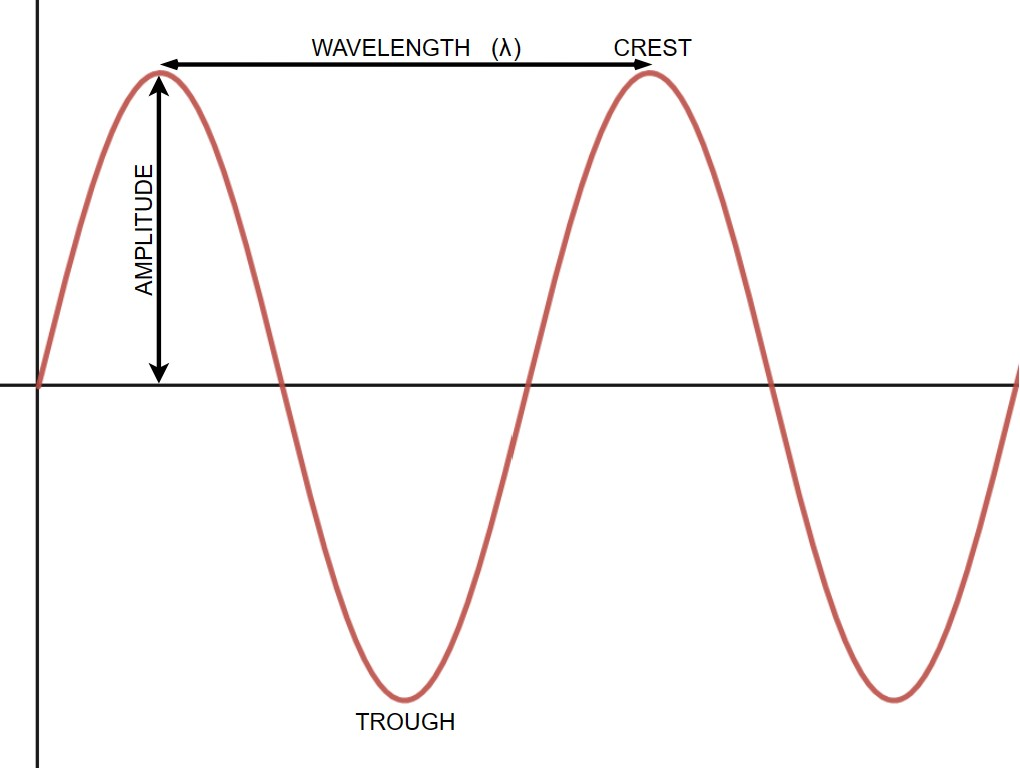
\includegraphics[width=\textwidth]{images/wave.jpg}
        \caption{Representation of a wave’s properties}
        \label{fig:wave}
    \end{subfigure}
    \hfill
    \begin{subfigure}{0.48\textwidth}
        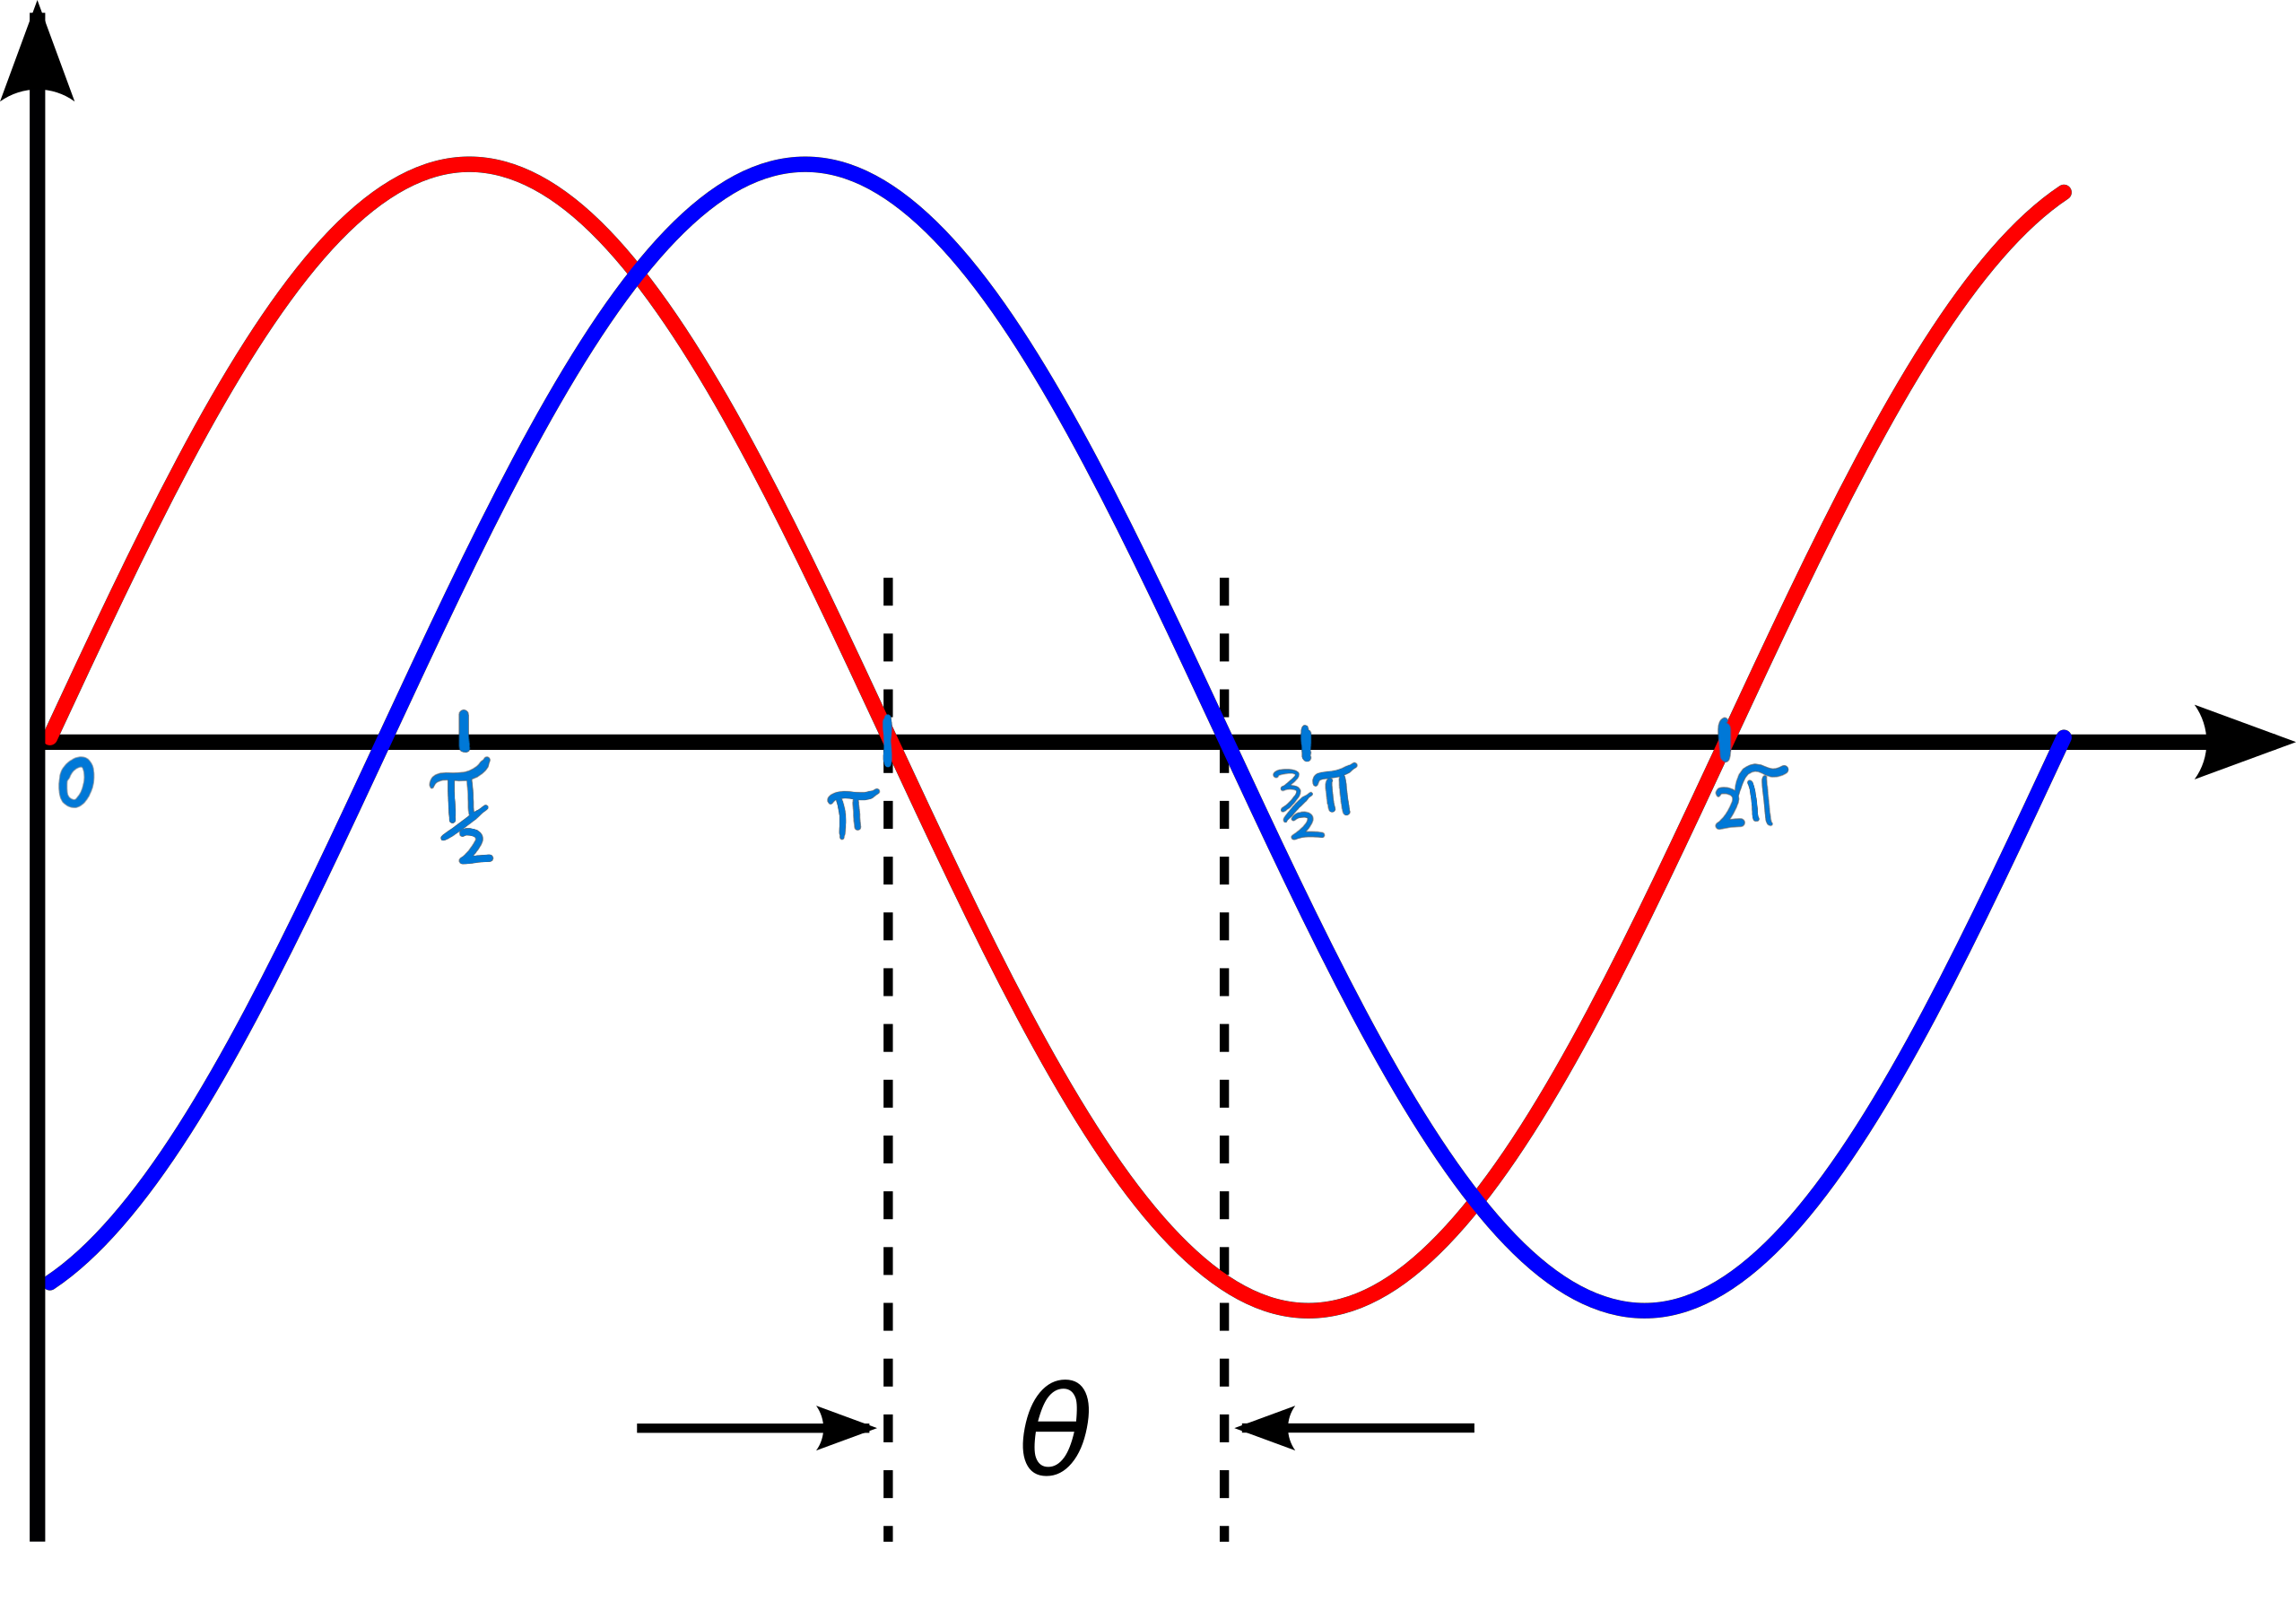
\includegraphics[width=\textwidth]{images/Phase_shift2.png}
        \caption{Illustration of a phase shift.}
        \label{fig:phase}
    \end{subfigure}
\end{figure}
The mathematical link between the frequency $f$, the wavelength $\lambda$, and the
wave propagation velocity $v$ is expressed as follows:
$$ f = \frac{v}{\lambda} $$
Where in vacuum $v = c$, the speed of light, as explained before. From the previous equation we get:
$$ v = f\lambda \qquad and \qquad \lambda = \frac{v}{f} $$
indicating how the frequency and wavelength of an EM wave are directly proportional to the propagation velocity and inversely proportional to each other.

The last key component used to describe a wave is the phase. The phase of a wave refers to its position within one complete cycle, describing how much of
the cycle has occurred at a specific point in space and time. It is often measured in radians or degrees, and it helps determine where a wave is in its
oscillation at a given moment. A phase angle of 0 represents the starting point of a cycle, while $2\pi$ (or 360°) corresponds to one complete cycle.
When comparing two waves, the phase difference, or phase shift, is the angular difference between their phase angles, and it indicates how "out of sync"
or "in sync" they are, as seen in Fig. \ref{fig:phase}. Considering two sinusoidal waves, when the phase difference is a multiple of $2\pi$, the addition
of the two waves results in a constructive interference, leading to reinforcement and a larger amplitude. Vice versa, destructive interference occurs when
the phase difference is an odd multiple of $\pi$, leading to cancellation and a smaller amplitude.

With those characteristic we can formulate the mathematical representation of a periodic wave, that tells us the momentary amplitude at instant $t$:
$$ a(t) = A\cos(2\pi ft + \phi) $$
made up of the following components:
\begin{itemize}[itemsep=1.5pt]
    \item $a(t)$: The instantaneous amplitude of the wave at time t.
    \item $A$: The amplitude of the wave, its maximum value.
    \item $2\pi f$: The angular frequency in $rad/s$, where $f$ is the frequency in Hertz ($1/s$)
    \item $t$: The time in seconds, indicating the instant at which you evaluate $a(t)$
    \item $\phi$: The phase offset, in radians, that determines the wave' starting position.
\end{itemize}
When $\phi$ is non-zero, the entire waveform appears to be shifted in time by $\frac{\phi}{2\pi f}$ seconds. A negative value represents a delay,
and a positive value represents an advance. The above equation describes a sinusoidal wave as a function of time, and it's a fundamental building
block in understanding and modeling periodic oscillations and waveforms in various fields of science.
\section{I/Q sampling}
\label{sec:IQ}
In many real-world applications, information is transmitted through analog signals, which vary continuously over time. To process and analyze these signals
using digital electronics, they need to be converted into a discrete digital form, a process known as sampling. I/Q sampling is a method used to sample
and represent a complex-valued analog signal, from which we can retrieve both amplitude and phase information. The "I" component represents the in-phase
or real part of the signal, while the "Q" component represents the quadrature or imaginary part of the signal. Denoting with $A$ the amplitude and with
$\phi_t$ the phase of the wave at instant $t$, we got:
$$ I(t) = A\cos(\phi_t) \qquad and \qquad Q(t) = A\sin(\phi_t)$$
Now, we can construct the complex number at any given time $t$ by combining the "I" and "Q" components
$$Z(t) = I(t) + jQ(t)$$
Where $j$ is the imaginary unit ($j^2 = -1$). Therefore, as depicted in Fig. \ref{fig:IQ_sample}, any sinusoidal wave can be
described by a composition of those two components (that is, by a single complex number), from which it is possible
to obtain the amplitude and the phase using the following equations:
$$ A = \sqrt{I(t)^2 + Q(t)^2} \qquad and \qquad \phi_t = atan2(I(t), Q(t)) $$
The first formula is simply the Pythagorean theorem applied to the two sides, in our case I and Q, to find the hypotenuse, that matches the amplitude.
The second one uses $atan2(x,y)$, a function that returns the angle formed by any vector [x, y] with the positive x-axis, bounded in the interval ($-\pi$, $\pi$].
The angle is positive if counterclockwise, negative if clockwise. Additionally, since $\cos(x) + j\sin(x) = e^{jx}$, we can represent the I/Q sample in the Euler's form:
$$Z(t) = A(\cos(\phi_t) + j\sin(\phi_t)) = Ae^{j\phi_t}$$
\begin{figure}[h]
    \centering
    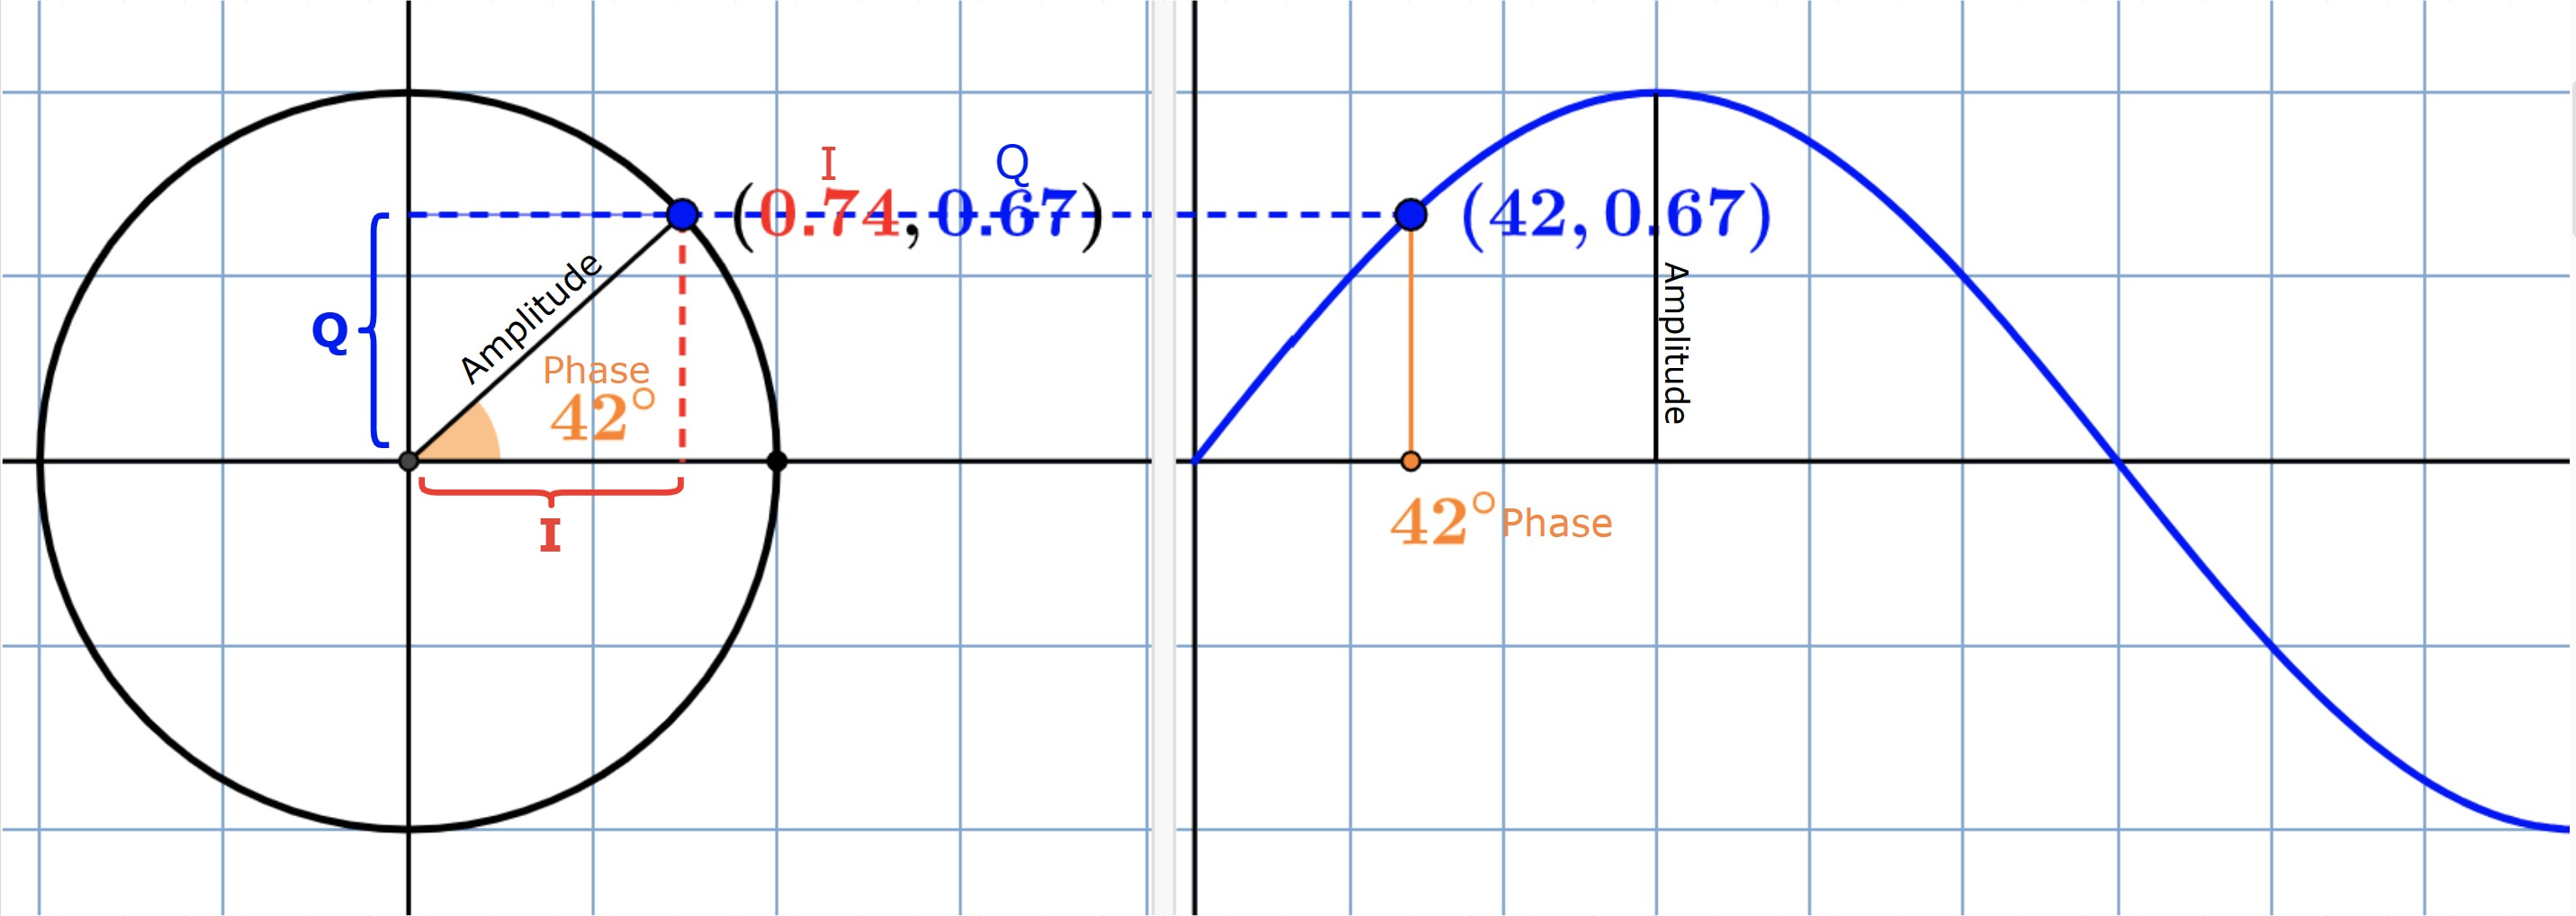
\includegraphics[width=0.96\textwidth]{images/IQ_sampling.jpg}
    \caption{Decomposition of a wave in I/Q components.}
    \label{fig:IQ_sample}
\end{figure}

\section{Orthogonal Frequency-Division Multiplexing}
Orthogonal frequency-division multiplexing (OFDM) is a modulation scheme used in wireless communication systems such as 802.11n
which encodes data streams into multiple overlapping subcarrier frequencies. In a traditional single-channel modulation scheme,
each data bit is sent serially or sequentially one after another. With OFDM a single information stream is split among several
closely spaced narrowband subchannel frequencies instead of a single Wideband channel \cite{OFDM_basics}. This enables each substream's
data rate to be lower than would be required by a single stream of similar bandwidth and makes the system less susceptible to corruption.
Even though the subchannel frequencies are closely spaced and do overlap to a degree,
they remain orthogonal, maintaining their distinct separation due to meticulous selection.
This strategy ensures that any interference is effectively negated.

OFDM signals are modelled in the frequency domain as the $sinc$ function:
$$sinc(f) = \frac{\sin(f)}{f}$$
The $sinc$ function has a central peak at zero frequency and then oscillates symmetrically around zero. It is characterized by its main lobe,
which contains most of its energy, and smaller side lobes that decrease in amplitude as you move away from the central peak, as seen in Fig.
\ref{fig:sinc_func}. The choice of the $sinc$ function is made due to its property of enabling orthogonal placement of each subcarrier with
respect to the others \cite{EdgeWiFiSensing2022}, as illustrated in Fig. \ref{fig:multiple_sinc} where five $sinc$ functions are strategically
positioned so that the primary subcarrier frequency (one is marked in red) coincides with a frequency at which all accompanying $sinc$ functions
assume a value of zero. This orthogonal configuration ensures that the summation of all five selected subcarriers maintains its peak values,
as presented in Fig. \ref{fig:summation}.
\begin{figure}[h!]
    \centering
    \begin{subfigure}{0.45\textwidth}
        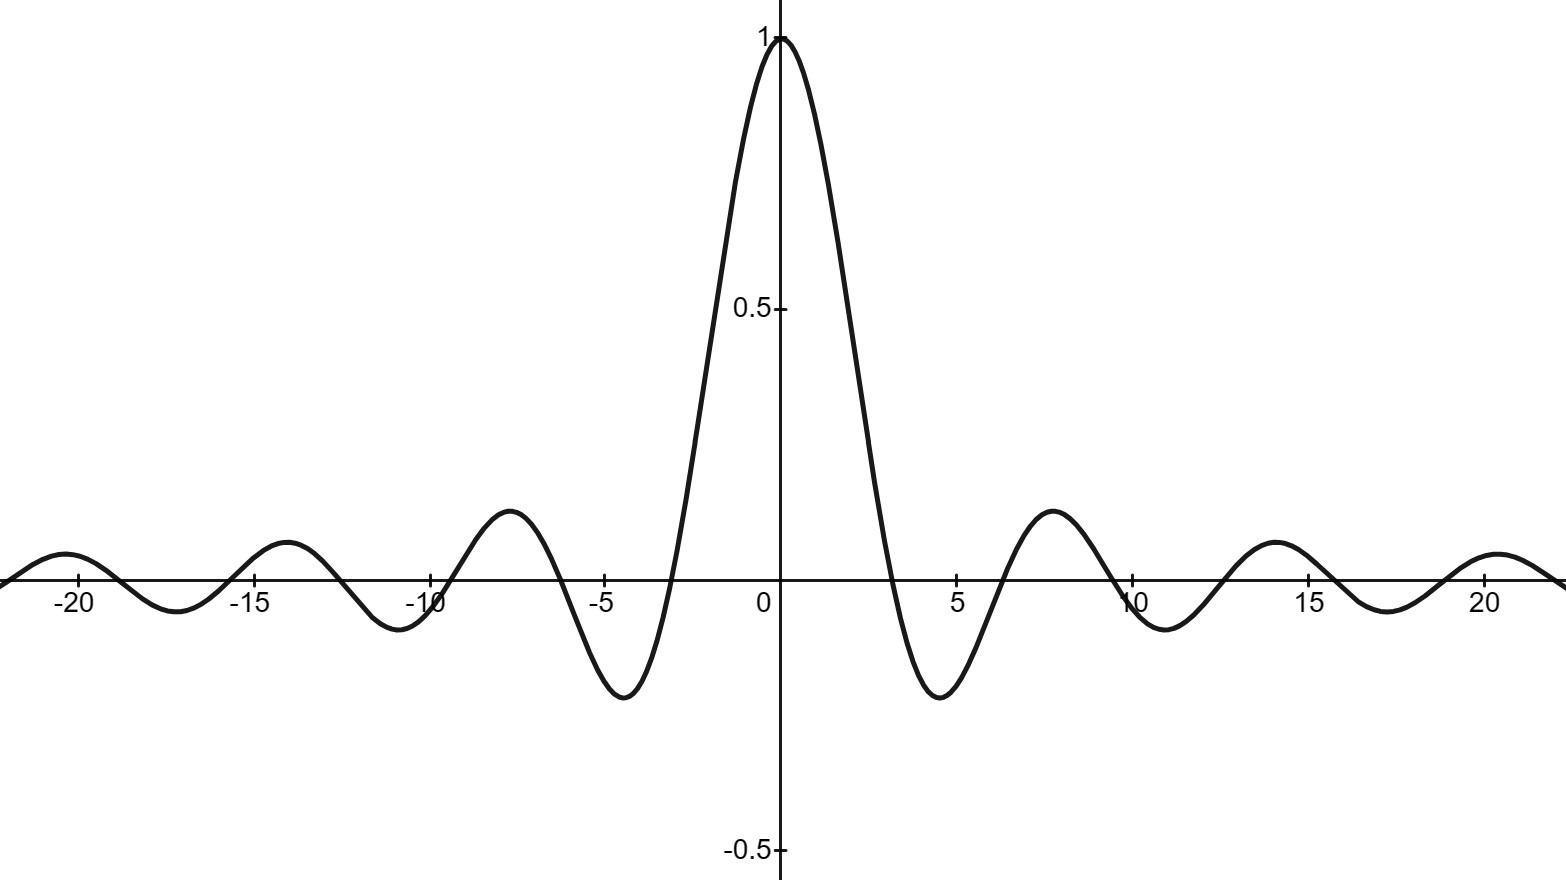
\includegraphics[width=\textwidth]{images/sinc_func_alone.jpg}
        \caption{The $sinc$ function for a single subcarrier signal.}
        \label{fig:sinc_func}
    \end{subfigure}
    \quad
    \begin{subfigure}{0.45\textwidth}
        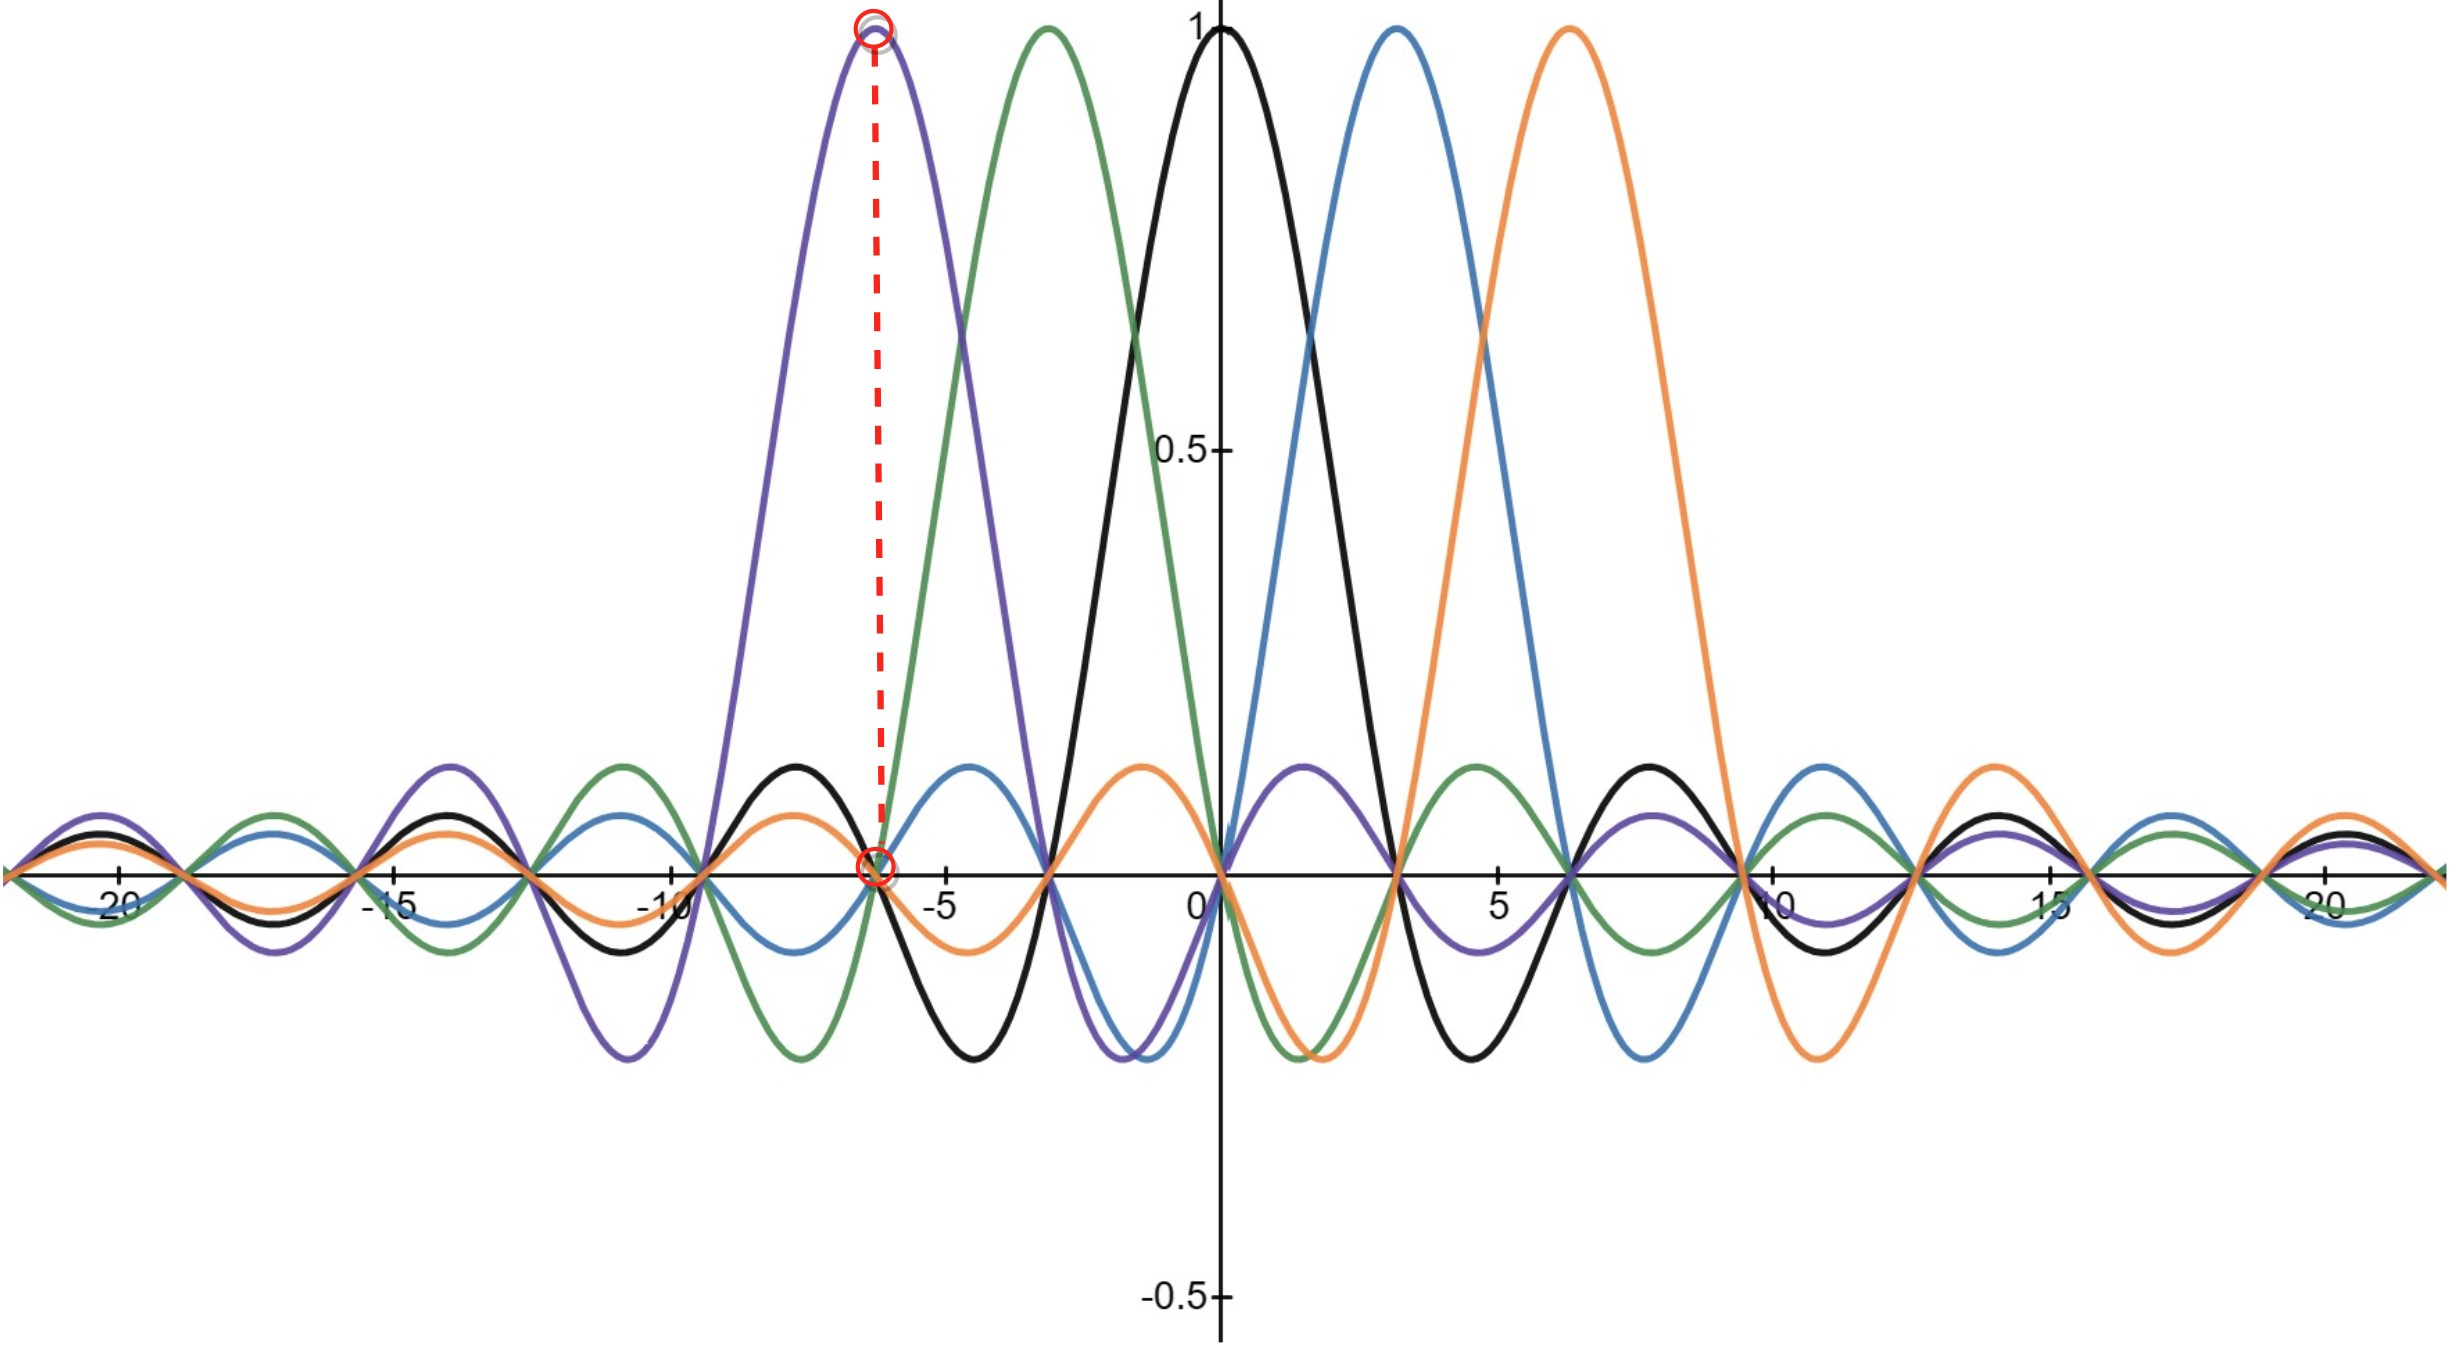
\includegraphics[width=\textwidth]{images/multiple_sinc.jpg}
        \caption{Orthogonal $sinc$ functions for multiple subcarriers.}
        \label{fig:multiple_sinc}
    \end{subfigure}
    \begin{subfigure}{0.45\textwidth}
        \centering
        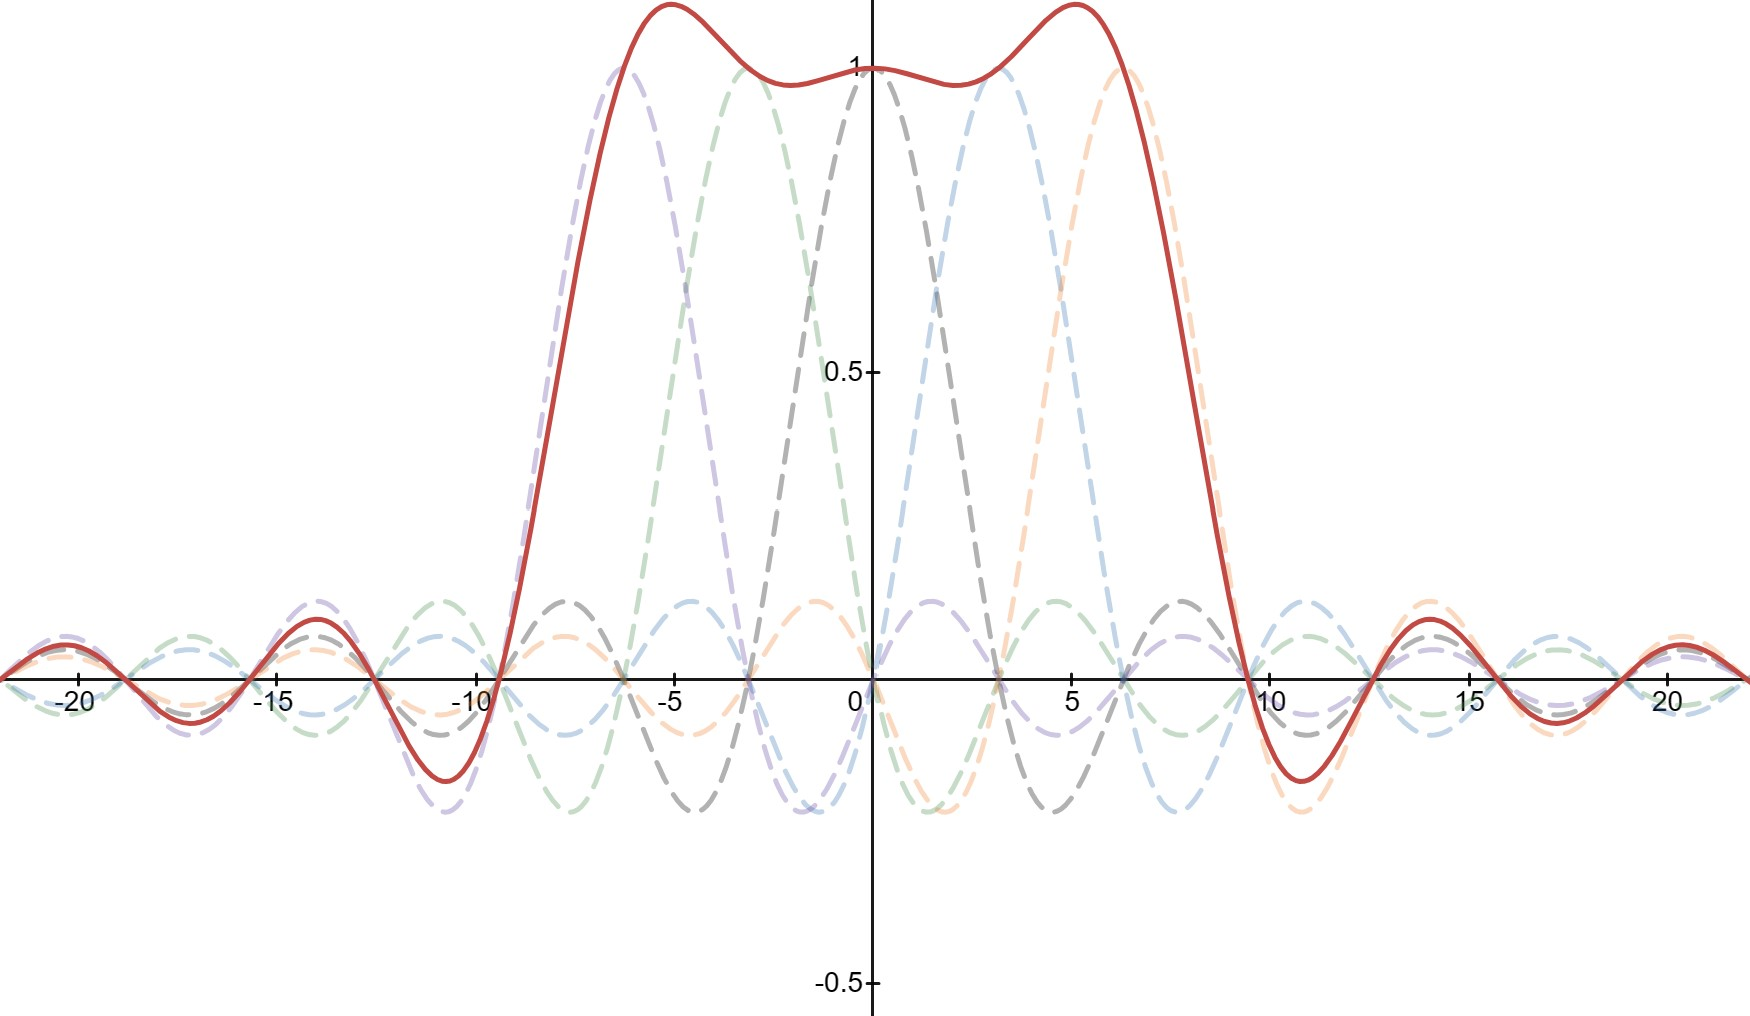
\includegraphics[width=\textwidth]{images/summationSinc.jpg}
        \caption{Signals summation.}
        \label{fig:summation}
    \end{subfigure}
\end{figure}

In order to transmit bits, a signal undergoes modulation. In wireless communication, modulation is the process of altering one or more characteristics
of a periodic waveform, called the carrier signal, with a separate signal called the modulation signal that typically contains information to be transmitted.
With OFDM, each subcarrier represents a single digital symbol that is being transmitted and can be modulated through various methods \cite{modulations} such
as Amplitude Shift Keying (ASK), Binary Phase-Shift Keying (BPSK) or Quadrature Amplitude Modulation (QAM). ASK involves switching the amplitude of the carrier
signal between two different levels (high and low) to represent binary data while BPSK achieves the same thing by altering the phase (usually $0^\circ$ and $180^\circ$)
to represent the travelling bits. QAM, widely used in Wi-Fi communication systems, combines instead both amplitude and phase modulation to convey multiple bits
of digital information in each modulation symbol, resulting in a higher data rate. Every OFDM symbol encodes binary data into a complex number by means of
$I/Q$ samples, as explained in Section \ref{sec:IQ}. For instance, 16-QAM has the capacity to express 4 bits of information using just one complex number \cite{QAM_explained}.

\section{Channel State Information}
CSI is the metric used in OFDM systems for describing amplitude and phase variations across subcarrier frequencies as wireless signals are transmitted
between a transmitter and a receiver. To detect these variations across subcarriers, OFDM systems transmit a set of known shared pilot symbols
(either interleaved in the transmitted message or as a preamble) which are then used to estimate the CSI vector H as:
$$y = H\odot x + \eta$$
where $y$ is a vector indicating the signal detected at the receiver, $x$ is the signal vector that was transmitted based on
the agreed upon pilot symbols, $\odot$ is the element-wise multiplication and finally $\eta$ is an additive white Gaussian noise vector.
$H$ is a complex vector containing a complex number (I and Q components) for each subcarrier representing the Channel Frequency Response (CFR),
from which we can retrieve the amplitude and phase of the specific subcarrier signal.
Throughout this work, two ESP32 microcontrollers are employed as TX and RX antennas \cite{ESP32_tool}, that perform OFDM communication with a bandwidth of 20MHz
using a total of 64 subcarriers. Multiple CSI samples are collected over a time window of size $W$, which can be represented as the $W\times S$ matrix

\[
    H = \begin{bmatrix}
        IQ_{11} & IQ_{12} & \dots  & IQ_{1S} \\
        IQ_{21} & \ddots  & \ddots & \vdots  \\
        \vdots  & \ddots  & \ddots & \vdots  \\
        IQ_{W1} & IQ_{W2} & \dots  & IQ_{WS}
    \end{bmatrix}
\]
\\
where S is the total number of subcarriers. In our case, 64 are employed, of which 12 are guard (null) subcarriers, resulting in having a final set of 52
usable informative subcarriers, at a rate of transmission of 100 packets (observations) per second.

\chapter{Signal Preprocessing}
\label{chap:preprocess}
This chapter explains the various methods used for preprocessing the available data, an essential procedure applied for structuring the dataset and
cleaning the CSI acquisitions, therefore making the system more robust and less susceptible to noise.

\section{Amplitude Sanitization}
\label{sec:amp_san}
During wireless transmissions, signal amplitudes can experience outliers or anomalies due to various factors and causes. These outliers can adversely
affect the quality of the received signal and the overall performance of the Wi-Fi system. Electrical spikes, equipment instability, external interference and
sudden movements in the environment are some possible sources of noise. To mitigate the effect of spurious data, the Hampel Filter \cite{hampel_ID, Gait_hampel_pca} is employed,
that exploits a sliding window and compares its central value with the Median Absolute Deviation (MAD), a robust statistical measure of the variability of a dataset defined as:
$$ MAD_{w} = Median\{\;|\,x - median(X_{w})\,|\quad \forall x \in X_{w}\;\} $$
where $X_{w}$ is a portion of the entire dataset defined by a sliding window $w$ of fixed length, where the length is an odd number. Then, the central point $x_{w/2}$ in the sliding window
is considered an outlier if:
$$|\,x_{w/2} - median(X_{w})\,|\; >\; \beta MAD_{w}$$
where $\beta$ is an application dependent hyperparameter: in our case $\beta = 3$, in alignment with the prevalent choice in the literature.
The detection procedure is performed independently on each subcarrier’s amplitude series, and every discovered outlier is substituted
with a prediction made by the Exponential Smoothing of the previous values in the window, to preserve temporal information consistency, formalized by:
$$s_0 = x_0$$
$$ s_{i+1} = \alpha x_i + (1-\alpha)s_i \quad \; \forall i \in [0,w/2)$$
Where $i$ indexes the samples in the first half of the window, $s_i$ is the smoothed value, $x_i$ is the observation and $\alpha$ is the smoothing factor.
A lower value of alpha gives more weight to past observations and produces a smoother forecast, while a higher value of alpha gives more weight to current observations and responds faster to changes.
In this work the value is set to $\alpha = 0.8$, but further testing and tuning could be required. For what regards the initial and last values of the dataset,
those that have a number of observations to their left or their right less than half of the window size, a static MAD filter is applied over the corresponding slices of size = $w/2 - 1$, and the outliers are substituted with the median.
As an extra relevant characteristic, the Hampel Identifier doesn't pose any strong assumption on the distribution of the data and works well even with non-normally distributed points. This is a clear distinction
with respect to other outlier detection statistical methods such as the Z-Score, that uses the mean and the standard deviation to discern anomalies
from the rest of the dataset. These measures assume that the data follows a symmetric Gaussian distribution, and they can be highly affected by skewness
or extreme outliers in case of non-normally distributed data. On the other hand, using the Median ensures resistance to skewness and to outliers with large
magnitude, and does not require any normality assumption.

The effect of the outlier removal procedure just described is the substitution of the most relevant outliers, but the series still preserve overall impurities causing large variance and heteroscedasticity.
To get rid of the noise, Discrete Wavelet Transforms (DWT) is employed, a common method for signal denoising. Other possible solutions include the application of a smoothing function, such as Weighted Moving Average and Exponential Smoothing,
but using more complex frequency based methods like Fourier Transforms and DWT is usually preferred. Fig. \ref{fig:Hampel1} shows the effect of applying Hampel Filtering with window size set to 51 and smoothing factor of 0.8 followed by DWT
to the amplitudes of subcarrier $12^{th}$. The DWT decomposes a signal into multiple scales using wavelet filters. High-frequency noise is concentrated in detail coefficients, while signal features are found in approximation coefficients.
By applying a threshold to detail coefficients that modifies them and reconstructing the signal with the inverse DWT, this technique effectively removes noise while preserving essential signal information \cite{DWT_review} at different frequency scales,
producing a smoothed version of the original data.

\begin{figure}[h]
    \centering
    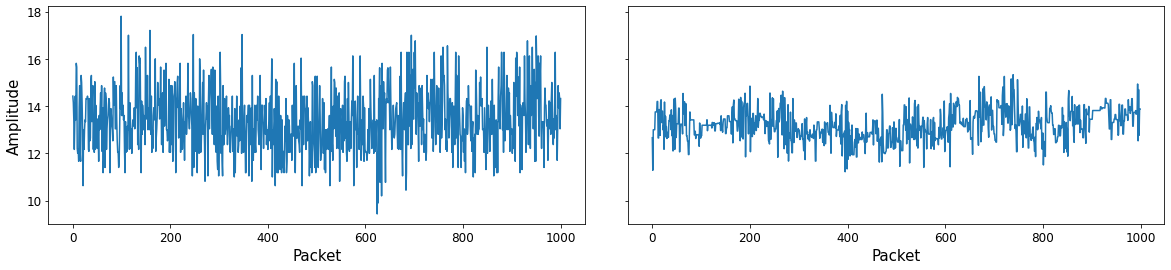
\includegraphics[width=0.98\textwidth]{images/hampel_DWT.png}
    \caption{Raw and filtered amplitudes of a single subcarrier over 10 seconds of acquisitions.}
    \label{fig:Hampel1}
\end{figure}

\section{Phase Sanitization}
\label{sec:cal}
Due to random noise and unsynchronized time clock between transmitter and receiver, raw phase information behaves extremely random, making it almost inapplicable for any task.
The issue is that phase data is affected by the carrier frequency offset (CFO) and sampling frequency offset (SFO) \cite{phase_noise}. The CFO arises when the transmitter and
receiver do not precisely synchronize their timing and phases before transmitting a packet, while the SFO is caused by analogue to digital converter, and it also varies by subcarrier, so each of them has a different
error in the end. The key observation is that significant component of random phase offsets can be removed by employing a linear transformation \cite{Phase_cal1,Phase_cal3} on the raw phase readings.
Indeed, the measured phase $\hat{\phi}_i$ for the $i^{th}$ subcarrier can be expressed as:
$$\hat{\phi}_i = {\phi}_i - 2\pi\frac{k_i}{N}\delta + \beta +\eta$$
where $\phi_i$ is the true phase, $\delta$ is the timing offset at the receiver that leads to the error expressed as the second term, $\beta$ is an unknown phase offset and $\eta$ is some measurement noise.
$k_i$ is the subcarrier index, ranging from -26 to +26 and N is the Fast Fourier Transform (FFT) size, a parameter found in the IEEE 802.11 specifications.
To mitigate the impact of random noises, linear transformation on the raw phases is performed. The key idea is to eliminate $\delta$ and $\beta$ by considering the phase across the entire frequency band. Firstly, we define two terms
$a$ and $b$ as follows:
$$ a = \frac{\hat{\phi}_n - \hat{\phi}_1}{k_n - k_1} \qquad \qquad b = \frac{1}{n}\sum_{j=1}^{n}\hat{\phi}_j$$
Subtracting the linear term $ak_i + b$ from the raw phase $\hat{\phi}_i$, we obtain a linear combination of true phases, denoted as $\Phi_i$, from which the random phase offsets have been removed (omitting the small measurement noise $\eta$):
$$\Phi_i = \hat{\phi}_i - ak_i - b $$
Fig. \ref{fig:phase_cal} illustrates an example of the phases after transformation, which distributes relatively stable as expected compared to the original random version. Although it cannot be claimed
the sanitized information is just the true phase, a usable and effective feature of the true phases is derived \cite{Phase_cal2}.
\begin{figure}[h]
    \centering
    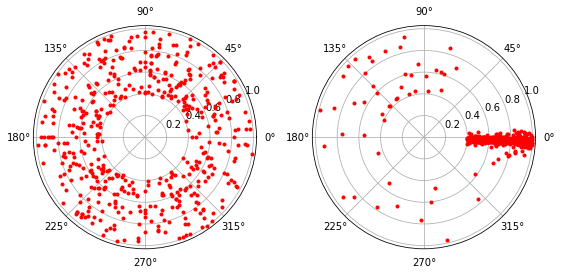
\includegraphics[width=0.9\textwidth]{images/phaseTransform.png}
    \caption{Raw and sanitized phases of subcarrier $9^{th}$ of 500 consecutive packets.}
    \label{fig:phase_cal}
\end{figure}
\section{Data exploration and structuring}
\label{Sec:structuring}
The main idea behind this work is that the presence of a human being in an area where a wireless communication is occurring,
distorts the EM waves in a unique manner, resulting in a person-specific CSI acquisition. Body characteristics such as shape, weight, mass distribution,
height, tissues and cellular composition have different levels of radiation absorption and reflection, affecting the phase and amplitude of the arriving signals.
This effect is of a particular magnitude if the distortion element, an object or a person, is located in the Line-Of-Sight (LOS) path between the communicating antennas.
This is because during a wireless transmission, the final signal is the result of a multipath propagation of the initial signal that is altered by the room structure and furniture,
but the LOS part of the wave usually overwhelms the other components coming from the multipath since it hasn't been affected by any object. Moreover, the transmission distance is the shortest
when considering the LOS with respect to other paths, leading to less signal fading and attenuation.

Fig. \ref{fig:heatmap} represents the amplitude of each subcarrier over time as a heatmap plot, where the scale goes incrementally from darker to lighter color, after the outlier filtering procedure describe in Section \ref{sec:amp_san}. The x-axis values are the different subcarriers,
ranging from index -26 to +26, while the y-axis represent the time steps for a total of 200 observations (2 seconds). The first image is the acquisition of a room with no person in it, while the second and third
images are the data of the same room but with a different person standing at the center of the LOS path. The empty room heatmap looks way more stable over time, with the amplitudes linearly decreasing
from the lowest subcarrier index to the highest one. This structure is more or less maintained whatever time frame it is selected. A person between the antennas instead, introduces notable noise caused by overall amplitude modifications,
with clear differences between two distinct people. Indeed, by analyzing the data points, it can be seen that the distribution of the amplitudes of each subcarrier for the empty room approximates quite well a Gaussian distribution, while on the other hand the distribution of the people-related data presents
irregularities and some skewness.
\begin{figure}[h]
    \centering
    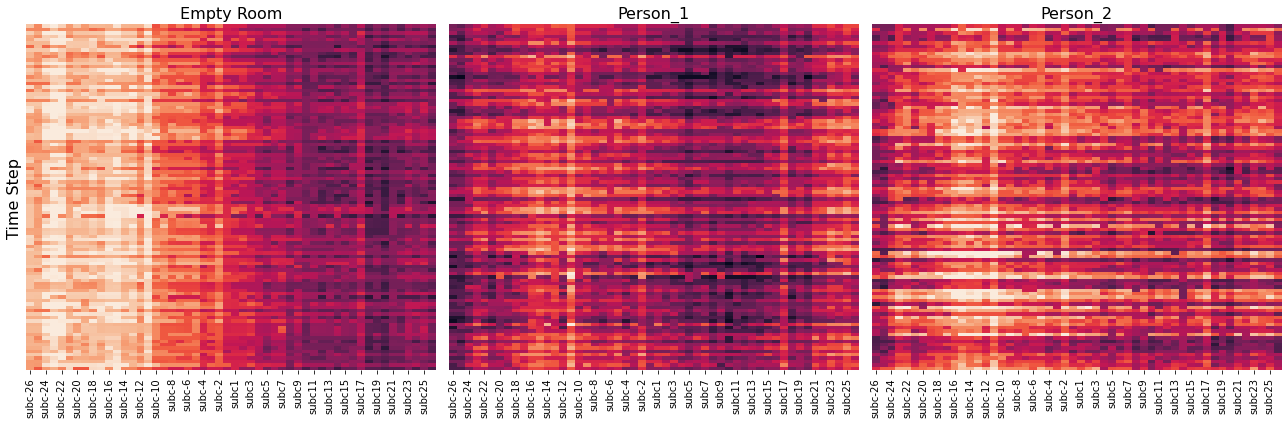
\includegraphics[width=0.95\textwidth]{images/heatmap_3.png}
    \caption{Heatmaps of the amplitudes of an empty room vs the same room with 2 different people standing in the LOS path between the antennas.}
    \label{fig:heatmap}
\end{figure}
For what regards the signal phases, visualizing the differences between classes is harder due to the angle-nature of the data and the calibration procedure explained in Section \ref{sec:cal}, that tends to normalize and center the points around the mean.
However, experimental results show a significant improvement in the classification task when combining both amplitude and phase information versus using the amplitude data alone, suggesting that also phases could be used to extract features that are
important for mapping signals to a specific person.

One logical approach to merge amplitude and phase data into a single data point is to create 2 different channels by concatenating them along the depth dimension, obtaining a tensor with shape $( 2 \times T \times S)$, where $T$ are the considered
time steps and $S$ the number of subcarriers, and passing it into a model ready to handle this kind of input shapes. Despite that, in this research an experimental method is tested, that consists into combining both measurements into a single
bi-dimensional image, by alternating amplitude and phase of their respective subcarriers. Precisely, if we indicate with $A_{ts}$ and $\phi_{ts}$ the amplitude and phase of subcarrier $s$ at time $t$ the image is constructed as follows:
\\
\[
    H = \begin{bmatrix}
        A_{11} & \phi_{11} & A_{12} & \phi_{12} & \dots  & \dots  & A_{1s} & \phi_{1s} \\
        A_{21} & \phi_{21} & \ddots & \ddots    & \ddots & \ddots & \vdots & \vdots    \\
        \vdots & \vdots    & \ddots & \ddots    & \ddots & \ddots & \vdots & \vdots    \\
        A_{t1} & \phi_{t1} & \dots  & \dots     & \dots  & \dots  & A_{ts} & \phi_{ts}
    \end{bmatrix}
\]
\\
getting a final image of shape $(T \times 2S)$. In this particular project, since 52 subcarriers are used and 200 time steps are observed, the shape of an input point is $(200 \times 104)$.
Since the acquired data consists of thousands of observations, to extract the various portions from the whole sequence a sliding window of length 200 moves along the series making steps of 100 points each time
and then the observations falling in the window are saved as a data point. This means that the entire series is not exactly divided in disjoint sections of length 200 each, rather in several portions where each one has the first half that overlaps with the
second half of the previous portion and consequently the second half that overlaps with first half of the next portion. To clarify, the extracted matrices are from row 0 to 200, 100 to 300, 200 to 400 and so on until the last row of the whole sequence.
The purpose of this mechanism is to capture the temporal dependencies between consecutive segments of the dataset, since during testing and inference any point in time could be captured without control over it. Furthermore, a form of data augmentation
is achieved as well, resulting into a larger training set.
\chapter{Proposed method}
This chapter explains the protocol followed for gathering the CSI data along with the architecture of the model employed for the classification task. A brief recap on CNNs is given, together with the description of the training settings and the dataset specifications, in order to build the complete working pipeline for the assigned task.
\section{Dataset acquisition}
The complete lack of public available CSI data designed for person Identification, brought the need of creating a brand-new original dataset. Some previous work \cite{WiWho_gait_decisionTree} tried to exploit the gait of the people to extrapolate their distinct features, hence the signal acquisitions
were done while the individual was roaming back and forth between the transmitting antenna (TX) and the receiving one (RX), walking at their custom pace. As opposite, the goal of this research is to identify people that are simply standing without requiring any specific movement pattern.
The CSI acquisition was done through the use of two ESP32 microboards, one set up for working as TX, the other as the RX. A total of 6 volunteers (regretting their choice) were involved, that have posed in all in the same room at different times. The room environment was kept exactly the same within the
whole dataset creation, without any change or displacement of furniture, objects or electronic devices. Each person was deprived of their phone that was kept in a different room, to prevent any chance of possible electromagnetic interference that would lead to twisted biometric data.
This was done to avoid spurious training and feature extraction: if the signal of a person was shaped by any foreign factor present only during the acquisition of that specific person, the model could learn to identify that class-unique factor rather than the person's biometrics.
The antennas were positioned at a distance of 3 meters one from the other, each connected to a laptop. The RX was programmed to collect the sampled data and save them directly into a file on its wired computer. Each person was asked to stand in the Line-Of-Sight of the antennas, precisely in the middle
point at 1.5 meters apart from the sides, facing a total of 6 different directions. In this way a variety of signal data corresponding to different body positions were gathered and analyzed with the goal of modelling dissimilar views of a person.
In Fig. \ref{fig:room} a view from above and a 3D render of the room setting is depicted, with the person facing the Transmitting device. The other 5 positions were the result of a 45$^\circ$, 135$^\circ$, 180$^\circ$, 225$^\circ$ and 315$^\circ$ rotation starting from the orientation shown in the image.
Each time, the subject was asked to remain still and breath normally, talking and minor movements were allowed, for a duration of 2 minute and 30 seconds. After the collection phase was terminated, the raw data were preprocessed and sanitized with the methods described in Chapter \ref{chap:preprocess}.
Since the packet rate was 100 pk/s and the overall duration considering all orientations was 15 minutes, a total amount of 90'000 observations per person were collected.
With the procedure explained in Section \ref{Sec:structuring} the final result is a dataset consisting in $\frac{90000 - 200}{100} + 1 = 899$ images for each class. The group of the 6 subjects was formed by 2 women with an average height, weight and age of 177cm, 66kg and 57 years, while the remaining 4 men were characterized by an average of
185cm, 84kg and 30 years of the respective statistics. In addition to the individuals, a CSI acquisition of the empty room with no people in it was acquired for study purposes.

\begin{figure}[t]
    \centering
    \begin{subfigure}{0.50\textwidth}
        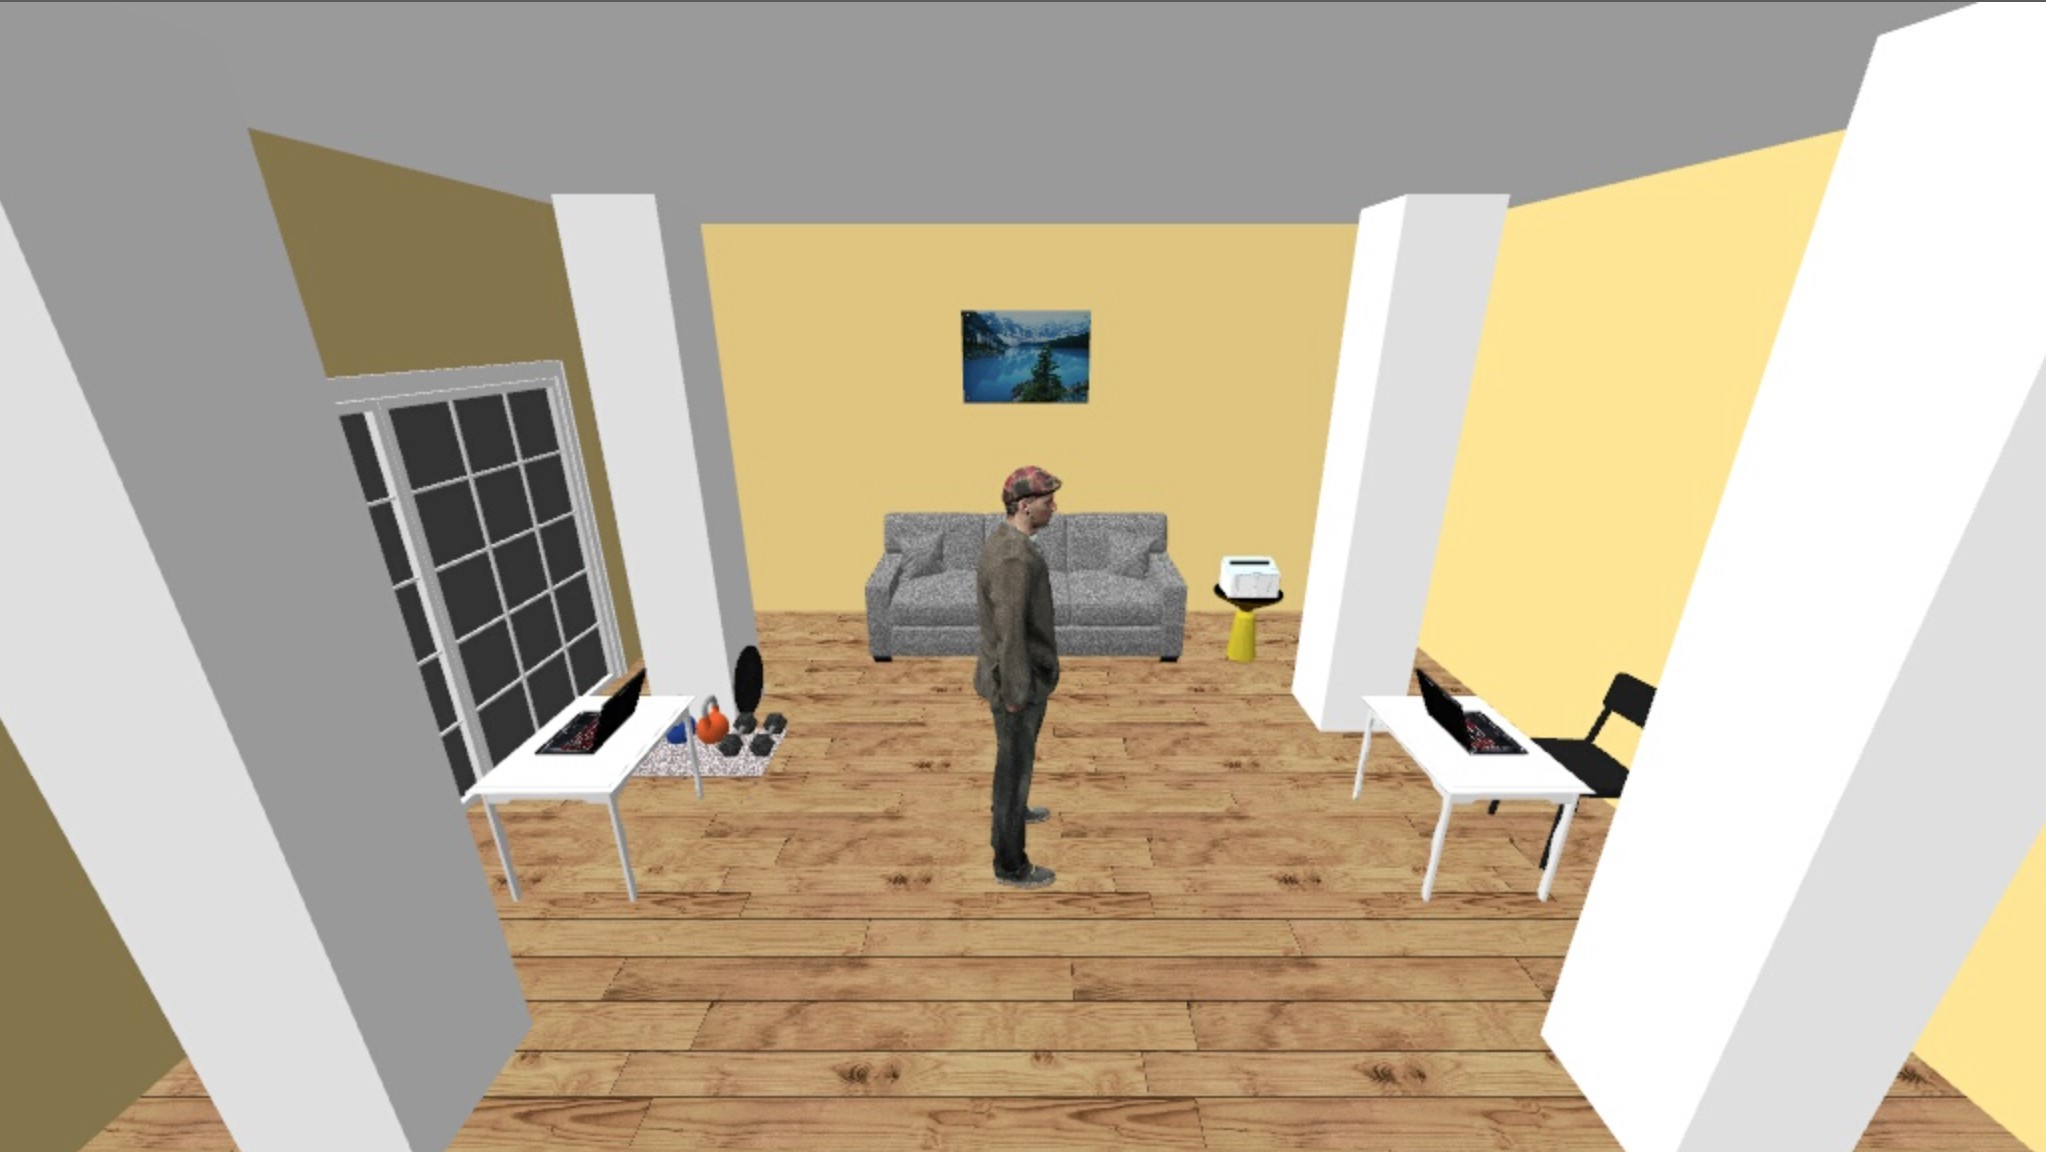
\includegraphics[width=\textwidth]{images/3D_room.jpg}
        \label{fig:3D_room}
    \end{subfigure}
    \quad
    \begin{subfigure}{0.40\textwidth}
        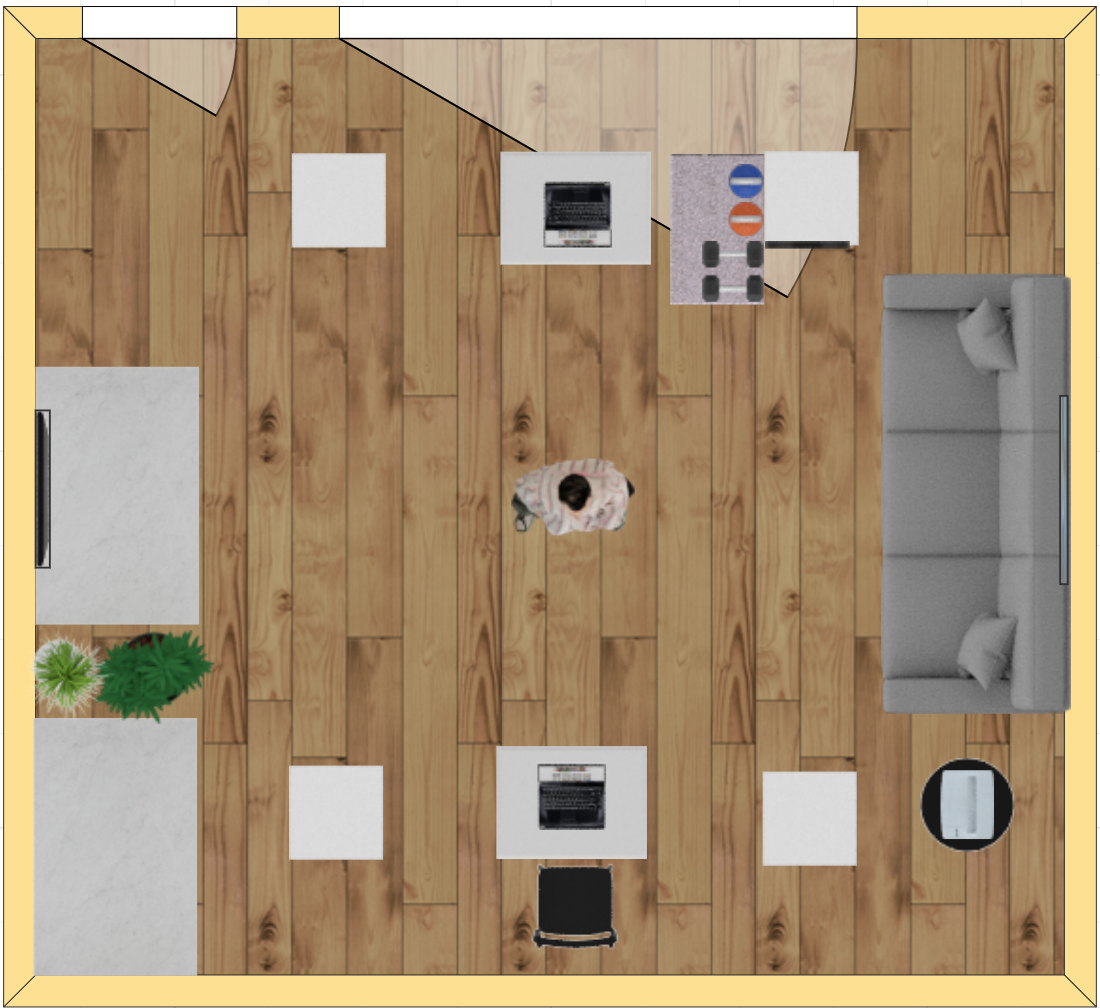
\includegraphics[width=\textwidth]{images/room2.png}
        \label{fig:2D_room}
    \end{subfigure}
    \caption{The room environment in which the data were taken (rendering).}
    \label{fig:room}
\end{figure}

\section{Convolutional Neural Network}
\label{sec:CNN}
One of the major breakthrough made in the deep learning history was the design of the Convolutional Neural Network (CNN) \cite{LeCun_CNN}, a specialized kind of neural network for
processing data that has a known grid-lie topology. Examples include time-series data \cite{time_conv,EEG_conv}, a 1-D grid taking samples at regular time intervals, and image data, a 2-D grid of pixels \cite{cnn_segment,class_cnn}.
CNN have been tremendously successful in a large pool of applications, becoming the Go-To architecture for a lot of common challenges. The characteristic operation of a CNN is the
Convolution, that adapted to grid-data structures consists into sliding a smaller matrix called Kernel on the input matrix and performing the sum of their element-wise products.
In many machine learning libraries the implementation, sometimes called "cross-correlation", can be mathematically formalized by:
$$S(i,j) = (K \ast I)(i,j) = \sum_{m}\sum_{n}I(i + m,j + n)K(m,n)$$
where $I$ is the input image, K is the kernel of size $m \times n$ and $s$ the output often referred as the "feature map". The latter has a size that is slightly smaller than the input,
since the operation shrinks the dimensions at the boundaries. A great property of convolutional layers is "translation equivariance" \cite{Goodfellow_DL}. Specifically,
a function $f(x)$ is equivariant to a function $g$ if $f(g(x)) = g(f(x))$. In case of image processing, that means the layer should be able to identify particular patterns,
such as edges, curves or more complex shapes in deeper levels of the net, wherever they are in the picture, even if shifted of some pixels.
This creates a 2-D map of where certain pattern are located in the original image. Similarly, when processing time-series data, this means that convolution produces a sort
of timeline that shows when different features appear in the temporal input. Since the nature of our data can be interpreted both as an image and a time-series (see Sec. \ref{Sec:structuring}),
a CNN is the proposed candidate for the job.
Another essential property of a CNN is the possession of sparse interactions (sometimes called sparse connectivity), as opposite to dense connectivity where each output is linked to every input features. This derives from the fact that the kernel is smaller than the input, for
instance within an image of millions of pixels it is possible to detect small meaningful features with kernels that occupy only tens of pixels. This reduces enormously the memory requirements,
since fewer parameter need to be stored, also boosting inference efficiency. If there are $m$ inputs and $n$ outputs, the matrix multiplication requires $m \times n$ parameters and the algorithm commonly used have $O(m \times n)$ running time.
Limiting the number of connection each output may have to $k$, then the sparsely connected methodology requires $k \times n$ parameters and $O(k \times n)$ runtime. The units of the input that are affected by the kernel to produce a single output point are known as
the Receptive Field of the point, enhanced in Fig. \ref{fig:rec_field}, accordingly to the same terminology used in optical science to describe region of the retina of the human eye activated by some visual stimulus. This make sense since several Artificial Intelligence algorithms originally take inspiration
from biology and the natural world, even though they end up to be completely different to biological systems.

\begin{figure}[h]
    \centering
    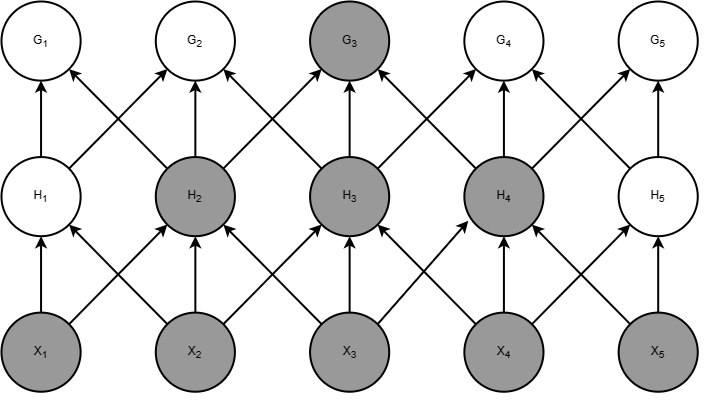
\includegraphics[width=0.8\textwidth]{images/convfield3.png}
    \caption{The receptive fields of the units in the deeper layers of a convolutional network is larger than the one of the units in the shallow layers.
        This effect increases with architectural features like pooling or strided convolutions. This means that even though direct connections are very sparse,
        units in the deeper layers \cite{rec_field} can be indirectly connected to most of the input tensor.}
    \label{fig:rec_field}
\end{figure}

\subsection{Pooling and Padding}
An ordinary convolutional block within a CNN comprises three phases. In the initial phase, the network conducts multiple parallel convolutions to generate a collection of linear activations.
Subsequently, each linear activation undergoes a non-linear activation operation, such as the rectified linear activation function or the sigmoid, in what is sometimes referred to as the detector stage.
Finally, in the third phase, a pooling operation is employed to further alter the layer's output.
A pooling function replaces the output of the net in a certain location with a summary statistic of nearby outputs \cite{pooling}. For example, the Max Pooling operation reports the maximum value within an input neighborhood.
It can be thought as a sliding kernel that returns the statistic instead of performing the convolution inner operation. Another popular pooling function is Average Pooling, that as the name says,
outputs the mean of the points falling in the window. In all cases, pooling helps to make the mapped representation nearly invariant to small translations of the original image, since the summary statistic should not change.
Because pooling summarizes the responses over a whole neighborhood, it is possible to use fewer pooling units than detector units, by reporting summary statistics for pooling regions spaced $k$ entries apart rather than 1 entry apart.
This improves the computational efficiency of the network because the next layer has roughly $s$ times fewer inputs to process. The number $s$ is called Stride, that is basically the step size of the sliding motion.
A common stride for the pooling layers is 2, that downsamples the input in roughly half of the initial dimensions. Precisely, the calculations for the dimensional transformation along a single axis go as follows:
$$out = \frac{in - k + 2p}{s} + 1$$
where $out$ and $in$ are the width or height of the output and input respectively, $k$ is the kernel width or height, $p$ is the padding and $s$ is the stride. The same formula holds for strided convolutions, since the shifting style is the same
of the pooling kernel, with just the operation that changes, and it is critical for constructing layers during design phase, when you must know how the feature maps' shapes vary.

The above-mentioned Padding is a technique used to control the spatial dimensions of the output feature maps after applying convolutional operations. It consists into adding extra rows and columns (or other axis) of zeros around the input data before applying the operation in the next layer.
Padding helps maintain the spatial dimensions of the input feature map as it passes through convolutional layers. Without padding, as you apply convolution operations, the spatial dimensions of the feature map tend to shrink with each layer, which may lead to a reduction
in the amount of information preserved. Padding prevents this reduction and can help preserve information at the edges of the input, even more useful if the dimensions of the input force the following pooling layer to ignore edge values
(for instance if the convolutional stride is even but the input size is odd). An example of the pooling operation with padded input can be visualized in Fig. \ref{fig:pooling}. There exist three particular cases of zero-padding setting that are worth mentioning \cite{padding_Conv}. One is the case in which no padding is used whatsoever, meaning that the kernel can visit
only positions where it is contained entirely within the input image: this is called \emph{Valid} convolution. With this choice, all pixels in the output are a function of the same number of pixels in the input. However, this leads to a smaller output size, limiting the number of convolutional
layers that can be included in the network, since the spatial dimension will eventually drop to $1 \times 1$. The second special case of zero padding is referred when enough zeros are added in such a way that the resulting feature map keeps the same size of the input matrix. This is usually called \emph{Same} convolution.
It does not limit the architectural possibilities of the next layers, but the input entries near the border influence fewer output entries than the ones near the center. After several convolutions, the cascade effect results into losing the boundary information of the input image.
The last method, referred as \emph{full} convolution, tries to avoid this effect by adding enough zeros for every pixel to be visited exactly $k$ times in each direction.

\begin{figure}[h]
    \centering
    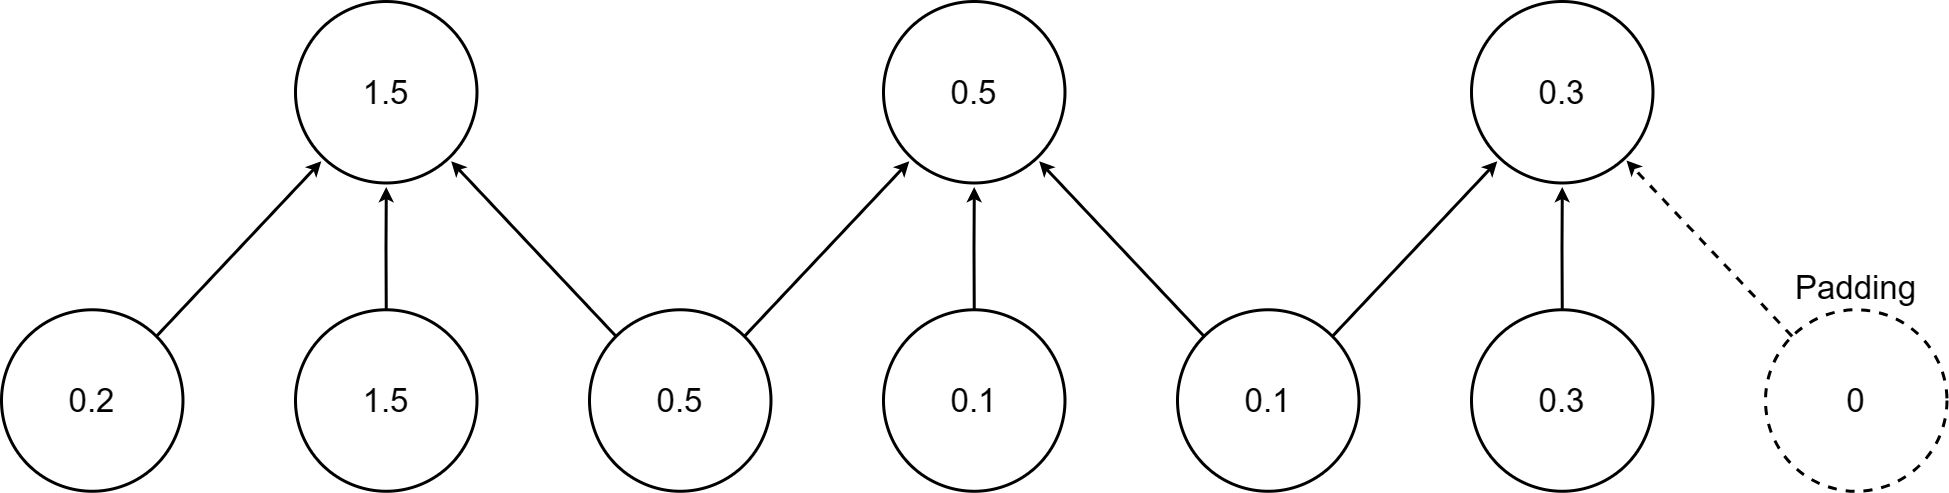
\includegraphics[width=0.82\textwidth]{images/poolingMax.png}
    \caption{A Max Pooling operation with a kernel of size 3 and stride between pools of 2. This reduces the representation size in a half, decreasing computational requirements while preserving the most important information. Note that the last pooling region on the right is zero padded, which can be just intended as a pooling kernel of smaller size, and must be included in order to not ignore border units.}
    \label{fig:pooling}
\end{figure}

\subsection{Dropout and Weight Decay}
\label{sec:dropout}
The remarkable capacity of deep neural networks to model intricate relationships in data also makes them susceptible to overfitting, a phenomenon where the model learns to memorize the training data rather than shaping the real data generating distribution. The general objective in machine learning is to find a bias-variance trade-off, a delicate balance between two sources of errors that affect a model's ability to generalize well to unseen data. Unfortunately,
very large and complex models such as Neural Networks tends to reduce the training bias up to a point where the accuracy on train set reaches 100\%, at the expense of variance that ends up being too large. This derives from the Universal Approximation Theorem, that explains how a shallow neural network has the capacity of approximating any continuous function up to any arbitrarily degree of precision, causing it to perfectly modelling the noise in the training set \cite{overfitting}.
Regularization for deep learning refers to a set of techniques and strategies designed to mitigate overfitting and improve the generalization capabilities. These strategies have been effectively used for decades prior to the advent of deep learning, with linear models like linear regression and logistic regression. Many regularization approaches are based on limiting the capacity of the models by adding a norm penalty $\Omega(\theta)$ to the loss function $J$, obtaining a regularized
loss function $\tilde{J}$:
$$\tilde{J}(\boldsymbol{\theta}; X, \boldsymbol{y}) = J(\boldsymbol{\theta}; X, \boldsymbol{y}) + \alpha\Omega(\boldsymbol{\theta})$$
where $\alpha \in [0, \infty)$ is a hyperparameter that weights the contribution of the norm penalty term $\Omega$ with respect to the standard loss function $J$. Larger values of $\alpha$ means more regularization, while $\alpha = 0$ results in no regularization at all.
During the training phase, minimizing $\tilde{J}$ will decrease both the original loss $J$ and some measure (the norm) of the size of the parameters $\theta$, or a subset of them if regularization is not applied globally but just on some layers.
A very popular penalty term is the $L^2$ norm, where $\Omega(\boldsymbol{\theta}) = \frac{1}{2}||\boldsymbol{\theta}||^{2}_{2} = \frac{1}{2}\boldsymbol{\theta}^\top\boldsymbol{\theta}$, commonly known as \emph{Weight Decay} regularization. This type of regularization drags the weights closer to the origin, since the $L^2$ vector norm can be intended as the Euclidean distance of a point from the origin.
Using the mentioned norm, the loss function obtained is:
$$\tilde{J}(\boldsymbol{\theta}; X, \boldsymbol{y}) = \frac{\alpha}{2}\boldsymbol{\theta}^\top\boldsymbol{\theta} + J(\boldsymbol{\theta}; X, \boldsymbol{y})$$
It follows the corresponding gradient with respect to the parameters:
$$\nabla_\theta\tilde{J}(\boldsymbol{\theta}; X, \boldsymbol{y}) = \alpha\boldsymbol{\theta} + \nabla_\theta J(\boldsymbol{\theta}; X, \boldsymbol{y})$$
By denoting the learning rate as $\lambda$, the gradient descent update rule for a single step then become:
$$\boldsymbol{\theta} \leftarrow \boldsymbol{\theta} - \lambda(\alpha\boldsymbol{\theta} + \nabla_\theta J(\boldsymbol{\theta}; X, \boldsymbol{y}))$$
that after a simple algebraic manipulation results in:
$$\boldsymbol{\theta} \leftarrow (1 - \lambda\alpha)\boldsymbol{\theta} - \lambda\nabla_\theta J(\boldsymbol{\theta}; X, \boldsymbol{y})$$
This shows how the addition of the weight decay term has modified the learning procedure to shrink the weight vector by a constant factor on each optimization step.
By reducing the magnitude of weights, $L^2$ regularization promotes a simpler model. A simpler model is more likely to generalize well to unseen data because it captures
the essential patterns in the data rather than fitting to the noise in the training dataset. Even more, this can make models less sensitive to outliers because it discourages
the parameters from assigning excessive importance to any single training point, leading to more robust model predictions. Following the same concepts, $L^1$ regularization
was designed, where the penalty term is indeed the $L^1$ norm: $\Omega(\boldsymbol{\theta}) = ||\boldsymbol{\theta}||_{1} = \sum_{i}|\theta_i|$, that is the sum of absolute value of
the individual components of the parameter vector. As before, $L^1$ weight decay controls the strength of regularization by using a factor $\alpha$ that scales $\Omega$:
$$\tilde{J}(\boldsymbol{\theta}; X, \boldsymbol{y}) = \alpha||\boldsymbol{\theta}||_1 + J(\boldsymbol{\theta}; X, \boldsymbol{y})$$
Similarly, \emph{Dropout} \cite{dropoput} provides a powerful regularization method without actually modifying the general formulas for the computations of the backward pass.
It works by randomly deactivating, or zeroing-out, a fraction of neurons during each training iteration. Each neuron in the layer has a probability, typically denoted as $p$,
of being temporarily deactivated, by multiplying by 0 the output of its activation function. The value of $p$ is a hyperparameter that determines the dropout rate or the fraction
of neurons to deactivate. During the backward pass, the gradients for the dropped-out neurons become effectively zero, a process that ensures that the network's weights are updated
based on the information from the active neurons only (a subset that changes at every step), thus preventing any single neuron from becoming too specialized to the training data.
Fig. \ref{fig:dropout} is an abstract representation of how a small network changes during a single step.
This regularization method can be interpreted as an approximation of performing \emph{bagging} over an ensemble of a great number of large neural networks, even though it is actually performed
on the same single network. Specifically, dropout trains the ensemble consisting of all subnetworks whose structure is obtained by removing the turned-off units from the underlying base architecture.
With bagging (short for bootstrap aggregating) $k$ different models are defined and $k$ different dataset are constructed by sampling from the training set with replacement (non-parametric bootstrap), and then finally
model $i$ is trained on dataset $i$. The predictions are consequently made by picking the most predicted class among the models, the so-called "consensus", or the average of the predictions for regression tasks.
Dropout aims to imitate this process but with an exponentially large number of neural networks.
\begin{figure}[h]
    \centering
    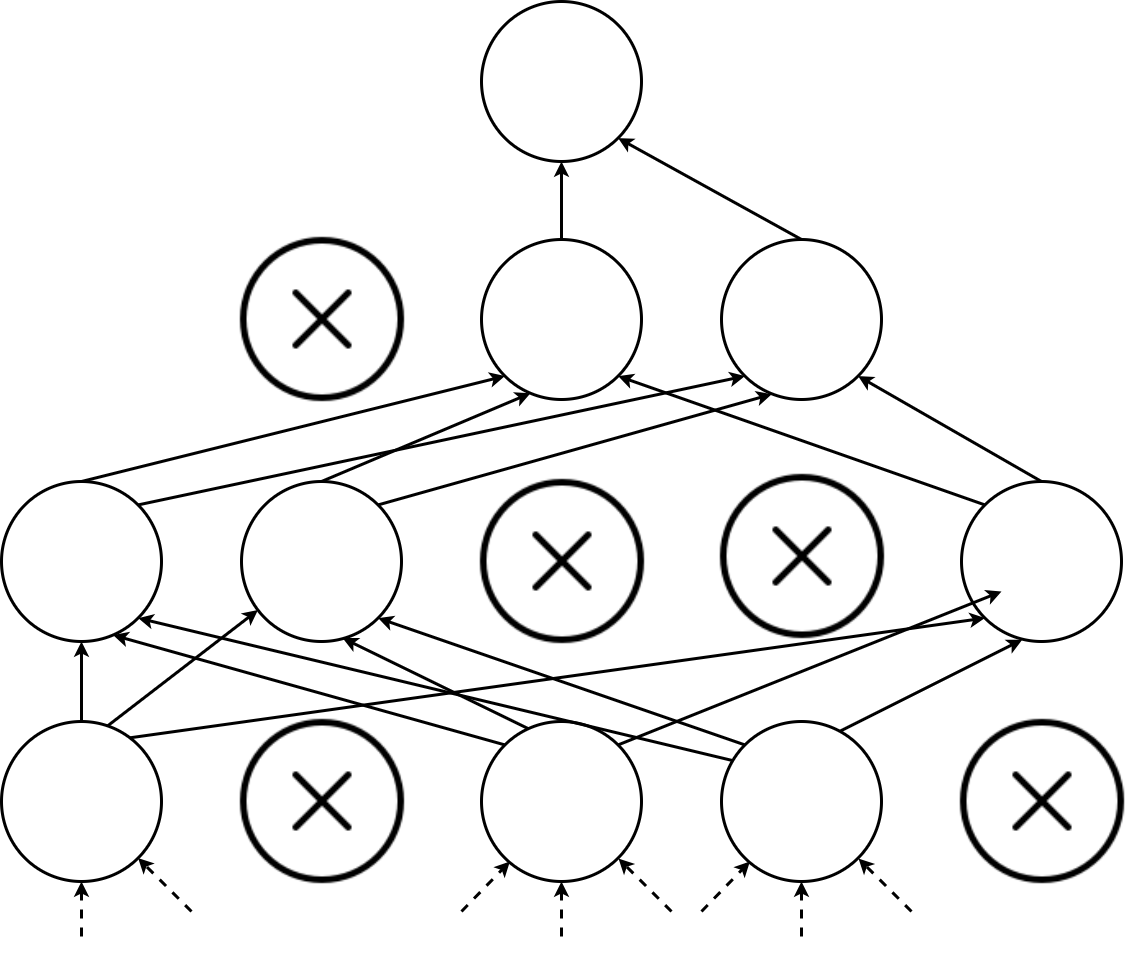
\includegraphics[width=0.5\textwidth]{images/dropout.png}
    \caption{A multilayer perceptron with dropout incorporated. Some units stochastically deactivate with probability $p$, creating a subnetwork that will be affected by backpropagation.
        At each update step, the units to be deactivated are resampled, obtaining new subnetworks time after time. This ensures that the model will not rely on just some "strong" neurons, but on a more
        distributed inference.}
    \label{fig:dropout}
\end{figure}
Specifically, training with dropout consists into using a minibatch-based algorithm such as stochastic gradient descent, that recalls the input bootstrap procedure of standard bagging methods. At each iteration,
a binary mask is applied to the hidden units (and, willingly, to the input too) that determines which units to deactivate. During testing phase, dropout is turned off, and the predictions are elaborated using
the full network architecture. Given that the process is stochastic, there is a chance that setting to zero some particular units, all paths that lead to the outputs will be deleted. But with Neural Network models that rely on
tens of layers and millions of units, the paths connecting the first and last layer are so many that this probability becomes insignificant. Many variants of Dropout have been proposed, such as \emph{Max Dropout} that sets the
probability $p$ based on the magnitude of the activation or \emph{Drop Connect} that drops individual connections (weights) rather than the entire unit, but in general terms, Dropout stays as one of the most effective regularization
technique \cite{regular_comparison}. It is finally observed that the best performances are often achieved by employing a combination of different regularization strategies \cite{regular_combining,survey_regular}, obtaining the greatest generalization ability.

\section{Proposed Architecture}
As anticipated, a Convolutional Neural Network model was designed to address the person Identification from Wi-Fi signals, as presented in Fig. \ref{fig:model}. Several reasons justify this choice. First, the data points are nothing more than sampled pieces of a multidimensional time-series,
structured as an image combining both amplitudes' heatmap and phase information and CNN are proved to be prodigious models when dealing with grid-like data. Moreover, as elucidated in Section. \ref{sec:CNN}, CNNs leverage shared weights and local receptive fields, allowing them to capture spatial
hierarchies and be translation invariant. This means that they can recognize patterns regardless of their position in the input, a property extremely useful when dealing with time frames extracted at any possible point in time. As a matter of fact, convolutional nets were already employed by recent work
regarding Human Activity Recognition \cite{cnn_csi_activity} and Indoor Localization \cite{cnn_csi_localization} using Wi-Fi derived CSI images, achieving remarkable results, suggesting that a CNN are worth to be tested also for CSI-based person ID.
\begin{figure}[h]
    \centering
    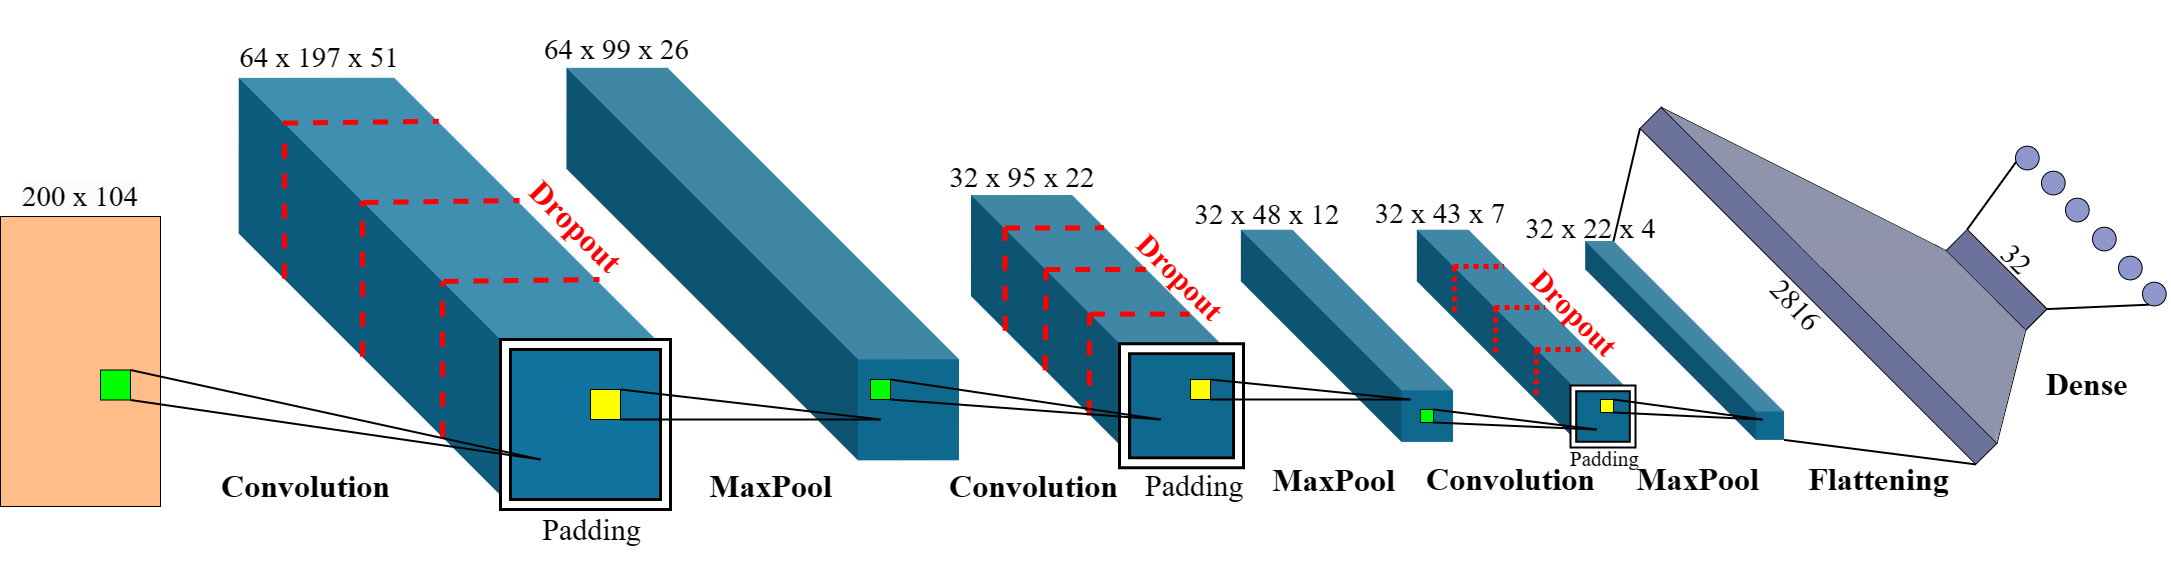
\includegraphics[width=\textwidth]{images/convNet.png}
    \caption{The Convolutional Neural Network architecture designed for the CSI-based person Identification task.
        The same model was employed for testing the performance with 2,3,4,5 and 6 classes by only adjusting the last fully connected output layer, while the rest
        of the architecture was always kept intact. The shapes, written above each feature map, refer to the tensors before applying any padding operation.}
    \label{fig:model}
\end{figure}

Of a particular interest is the first convolutional layer, that transforms the image into 64 feature maps. The operation is done with a kernel of size $4 \times 4$ and a stride of 2 on the horizontal axis. The stride value was precisely selected due to the structure of the input image, defined in Section \ref{Sec:structuring}.
The features are the amplitude and phase of each subcarrier positioned in an alternating style, in such a way that every couple of columns represents amplitude and phase of the same subcarrier. Using a stride equals 2 makes the filters jumping couple after couple, considering subcarrier after subcarrier.
To be precise, given that the kernel shape is four by four, two subcarriers are considered on each filter multiplication, in a time range of 4 observations. This method brings two nice outcomes: primarily, the amplitude information of a subcarrier is never divided by its corresponding phase information, capturing the whole signal
description; Secondly, each individual weight of the kernel is always multiplying the same nature of data, since it never slides making single steps, so that weights $w_{11}, w_{13}, w_{21}, w_{23}$ on the 4 by 4 filters constantly refer to amplitude numbers while weights $w_{12}, w_{14}, w_{22}, w_{24}$ always encounter phase data.
Even though those properties could somewhat be obtained using the standard double-channel input image fabric, it would be academically engaging to see a performance comparison between the two ideas, but it was out of the scope of this research.
After having discussed the architectural choices of the first convolution, the settings of each layer of the presented neural network are selected as follows:

\begin{enumerate}
    \item \textbf{Input}: $200 \times 104$ image combining signal data.
    \item \textbf{Convolution + Dropout}: Kernel size = $4 \times 4$, stride = (1, 2), output channels = 64, dropout $p$ = 0.3, resulting dimensions = $64 \times 197 \times 51$.
    \item \textbf{Padding + Max Pooling}: Padding = 1, Kernel size = $2 \times 2$, stride = 2, resulting dimensions = $64 \times 99 \times 26$.
    \item \textbf{Convolution + Dropout}: Kernel size = $6 \times 6$, stride = (1,1), output channels = 32, dropout $p$ = 0.3, resulting dimensions = $32 \times 95 \times 22$.
    \item \textbf{Padding + Max Pooling}: Same as before, resulting dimensions = $32 \times 48 \times 12$
    \item \textbf{Convolution + Dropout}: Kernel size = $6 \times 6$, stride = (1,1), output channels = 32, dropout $p$ = 0.3, resulting dimensions = $32 \times 43 \times 7$.
    \item \textbf{Padding + Max Pooling}: Same as before, resulting dimensions = $32 \times 22 \times 4$
    \item \textbf{Flattening + Fully Connected}: Resulting dimension = 2816 to 32 to 6 output classes.
\end{enumerate}
Dropout here refers to \emph{Spatial Dropout}, also called 2-D Dropout, that works by randomly deactivating not single units but an entire feature map (or channel).
The choice of the Dropout probability rate (see subsection \ref{sec:dropout}) was dictated by trials and testing, after which 0.3 seemed to retain a good model in terms of validation accuracy.
Max Pooling was harnessed to get downsampled feature maps, together with padding to ensure boundaries points were included. At the end, two fully connected layers are present to map the features
extracted by the previous convolutions to an output class. The activation function used in all layers was the Rectified Linear Unit (ReLU), the most common choice nowadays, that boost convergence
time and increase overall sparsity.

\chapter{Results}

\bibliography{references}
\bibliographystyle{ieeetr}

\end{document}
